\documentclass[11pt,a4paper]{article}

\usepackage[margin=2.5cm]{geometry}
\usepackage{setspace}
\usepackage{hyperref}
\usepackage{titlesec}
\usepackage{parskip}
\usepackage{amsmath}
\usepackage{amssymb}
\usepackage{graphicx}
\usepackage{booktabs}
\usepackage{float}
\usepackage[utf8]{inputenc}
\setstretch{1.15}

\titleformat{\section}{\large\bfseries}{\thesection}{1em}{}
\titleformat{\subsection}{\normalsize\bfseries}{\thesubsection}{1em}{}

\title{First Stage Evaluation\\[0.3cm]
\large Non-Linear Mode Connectivity in Neural Networks\\and the Role of Permutation Symmetry}
\author{Maciek Lodzinski\\[0.2cm]
\small Supervisors: Dr. Jing Sun, Dr. David Tax\\
\small Delft University of Technology}
\date{January 2026}

\begin{document}

\maketitle

\tableofcontents
\newpage

\section{Project Overview}

Neural networks trained from different random initializations converge to distinct minima (modes) in the loss landscape. Mode connectivity investigates whether these modes can be connected by continuous paths along which the loss remains low. Garipov et al.\ (2018) demonstrated that such low-loss paths exist when parameterized as B\'{e}zier curves, enabling practical applications such as fast model ensembling and improved understanding of the loss landscape geometry.

A closely related line of research concerns permutation symmetry: neural networks are invariant to permutations of neurons within hidden layers, meaning that functionally identical networks can occupy different locations in parameter space. Entezari et al.\ (2021) conjectured that most SGD solutions can be permuted so that there is no barrier on the linear interpolation between them. This suggests that the loss landscape may be fundamentally simpler than it appears, with apparently distinct basins being permutations of the same underlying solution.

This thesis project combines both perspectives, investigating mode connectivity through multiple path-finding methods while exploring how permutation symmetry relates to the geometry of low-loss paths in order to better understand the loss landscape of neural networks.

\section{Thesis Overview: Testing the One-Basin Hypothesis}

\subsection{Aim and Central Question}

\begin{quote}
If two neural networks are trained from different random initializations on the same data, do they converge to solutions in the same basin of the loss landscape (modulo permutation symmetries)?
\end{quote}

This is often referred to as the \textbf{one-basin hypothesis} or the \textbf{Entezari conjecture}. In this framing, differences between independently trained solutions should be explainable primarily by neuron permutations, implying that a suitable alignment would yield negligible loss barriers under linear interpolation.

\subsection{Key Definitions}

\paragraph{Loss barrier (Frankle et al.\ 2020).}
Given two parameter vectors $\theta_A$ and $\theta_B$ with comparable loss, the \textbf{loss barrier} is defined as
\[
\text{barrier}(\theta_A, \theta_B) = \max_{\lambda \in [0,1]} \mathcal{L}\!\left((1-\lambda)\theta_A + \lambda \theta_B\right)
 - \frac{1}{2}\left(\mathcal{L}(\theta_A) + \mathcal{L}(\theta_B)\right),
\]
where $\mathcal{L}$ is the loss function (e.g., cross-entropy). The barrier is non-negative by definition and is typically approximated by evaluating the loss on a finite grid of interpolation points (Section~\ref{sec:evaluation-protocol}).

\paragraph{Linear mode connectivity (LMC).}
Two networks are \textbf{linearly mode connected} if their loss barrier is approximately zero:
\[
\text{barrier}(\theta_A, \theta_B) \approx 0,
\]
equivalently, if the loss along the linear interpolation remains close to the endpoint losses for all $\lambda \in [0,1]$.

\paragraph{Same basin (mode connectivity).}
Two solutions $\theta_A$ and $\theta_B$ are in the same basin if there exists a continuous path $\gamma : [0,1] \to \Theta$ with $\gamma(0)=\theta_A$ and $\gamma(1)=\theta_B$ such that
\[
\mathcal{L}(\gamma(t)) \approx \mathcal{L}(\theta_A) \approx \mathcal{L}(\theta_B) \quad \forall\, t \in [0,1].
\]
Mode connectivity (Draxler et al., 2018; Garipov et al., 2018) studies the existence and structure of such low-loss paths.

\paragraph{Interpretation.}
\begin{itemize}
    \item \textbf{Barrier $\approx 0$:} Flat or convex interpolation (connected).
    \item \textbf{Barrier $> 0$:} A loss ``hill'' between solutions (disconnected in linear space).
    \item \textbf{Barrier near random-init loss:} Strongly disconnected solutions.
\end{itemize}

\subsection{Permutation Symmetry and LMC Modulo Permutation}

Neural networks exhibit permutation symmetry: reordering neurons within a hidden layer (with corresponding weight adjustments) does not change the function. For a two-layer network $f(x) = W_2 \sigma(W_1 x)$ and a permutation matrix $P$ over hidden units,
\[
f(x) = (W_2 P^{-1})\, \sigma(P W_1 x) = W_2 \sigma(W_1 x),
\]
so the function is unchanged even though the parameters differ. For an $L$-layer network, the set of valid layer-wise permutations is
\[
\mathcal{P} = \{(P_1, P_2, \ldots, P_{L-1}) : P_\ell \in S_{n_\ell}\},
\]
where $S_{n_\ell}$ is the symmetric group on $n_\ell$ neurons in layer $\ell$.

\textbf{LMC modulo permutation:} two solutions are linearly mode connected modulo permutation if there exists $P \in \mathcal{P}$ such that
\[
\text{barrier}(\theta_A, P(\theta_B)) \approx 0.
\]

\subsection{Formal Statement of the One-Basin Hypothesis}

Entezari et al.\ (2021) conjecture that most SGD solutions belong to a set whose elements can be permuted so that linear interpolation has no barrier. Formally, for most pairs of SGD solutions $\theta_A, \theta_B$,
\[
\exists\, P \in \mathcal{P} \text{ such that } \text{barrier}(\theta_A, P(\theta_B)) \approx 0.
\]

\subsection{Hierarchy of Connectivity Claims}

\begin{table}[H]
    \centering
    \caption{Hierarchy of connectivity claims and current evidence.}
    \begin{tabular}{l l l}
        \toprule
        \textbf{Claim} & \textbf{Statement} & \textbf{Status} \\
        \midrule
        Mode connectivity (curved paths) & $\exists$ low-loss path between minima & Proven (Draxler, Garipov) \\
        LMC after shared training & Linear path has low barrier & Proven (Frankle) \\
        LMC modulo permutation & $\exists P$ s.t.\ linear barrier is low & Open (Entezari) \\
        LMC without alignment & Linear path between raw solutions is flat & Generally false \\
        \bottomrule
    \end{tabular}
\end{table}

\section{Research Questions and Scope}

The project addresses the following research questions:

\begin{enumerate}
    \item \textbf{RQ1:} How do different path-finding methods (B\'{e}zier curves, polygon chains, symmetry plane constrained paths) compare in terms of barrier height and path quality?
    \item \textbf{RQ2:} What is the role of permutation symmetry in mode connectivity? Do paths between permutation-equivalent modes differ from paths between independently trained modes?
    \item \textbf{RQ3:} Does constraining optimization to specific hyperplanes (e.g., the perpendicular bisector between endpoints) affect the quality of low-loss paths?
    \item \textbf{RQ4:} How robust is mode connectivity to variations in initialization, regularization, and architectural choices?
    \item \textbf{RQ5:} Are existing permutation-finding methods too weak or is the mode-permutation hypothesis incorrect?
\end{enumerate}

\textbf{Scope:} Experiments are conducted on two architectures---VGG16 ($\sim$15M parameters) and ConvFC---and two datasets---CIFAR-10 and Fashion-MNIST. Three independently trained models (seed0, seed1, seed2) serve as endpoints, along with mirror networks created via full neuron permutation.

\begin{figure}[H]
    \centering
    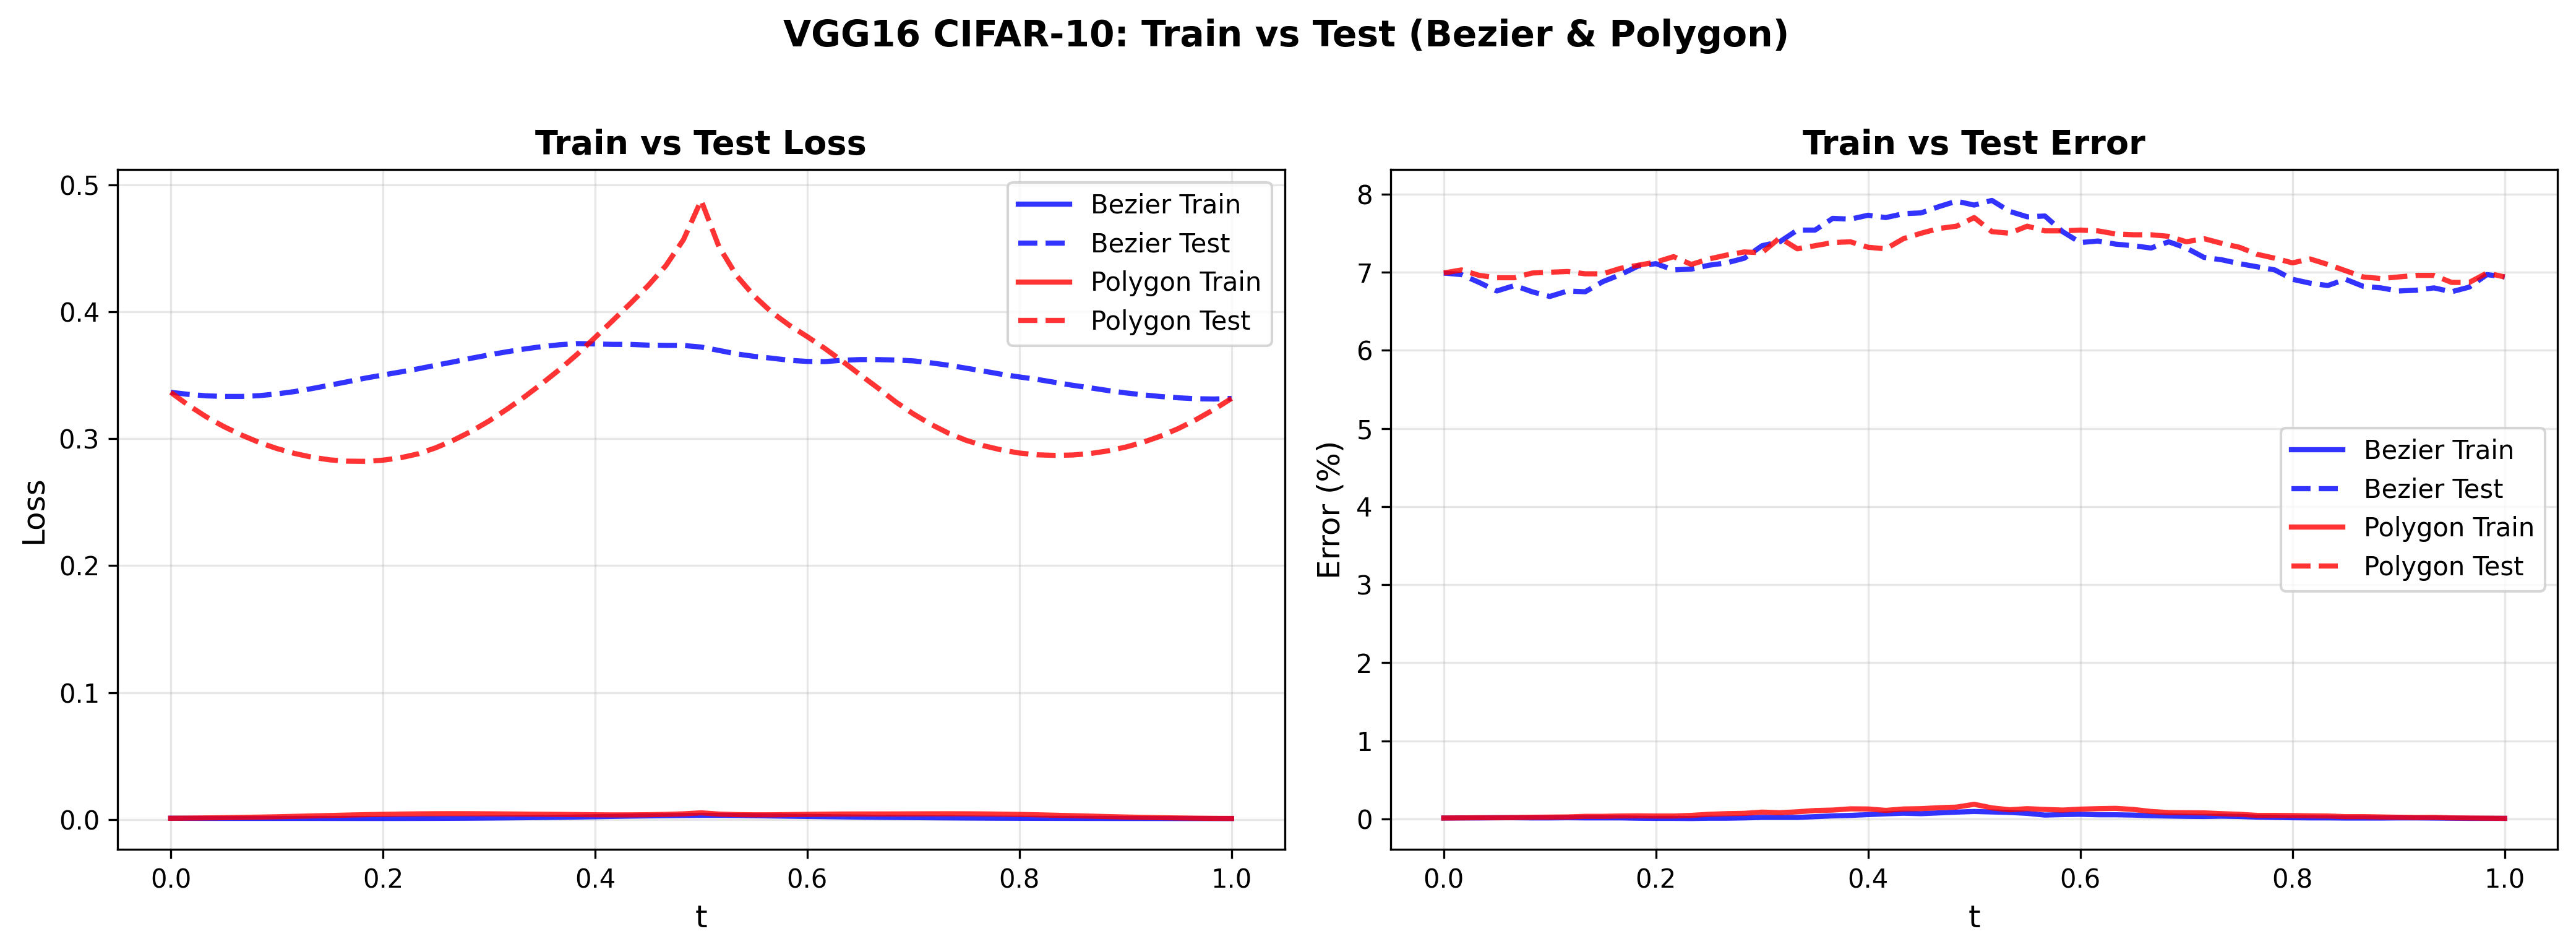
\includegraphics[width=0.95\linewidth]{../draft_3/vgg16.png}\\[0.5em]
    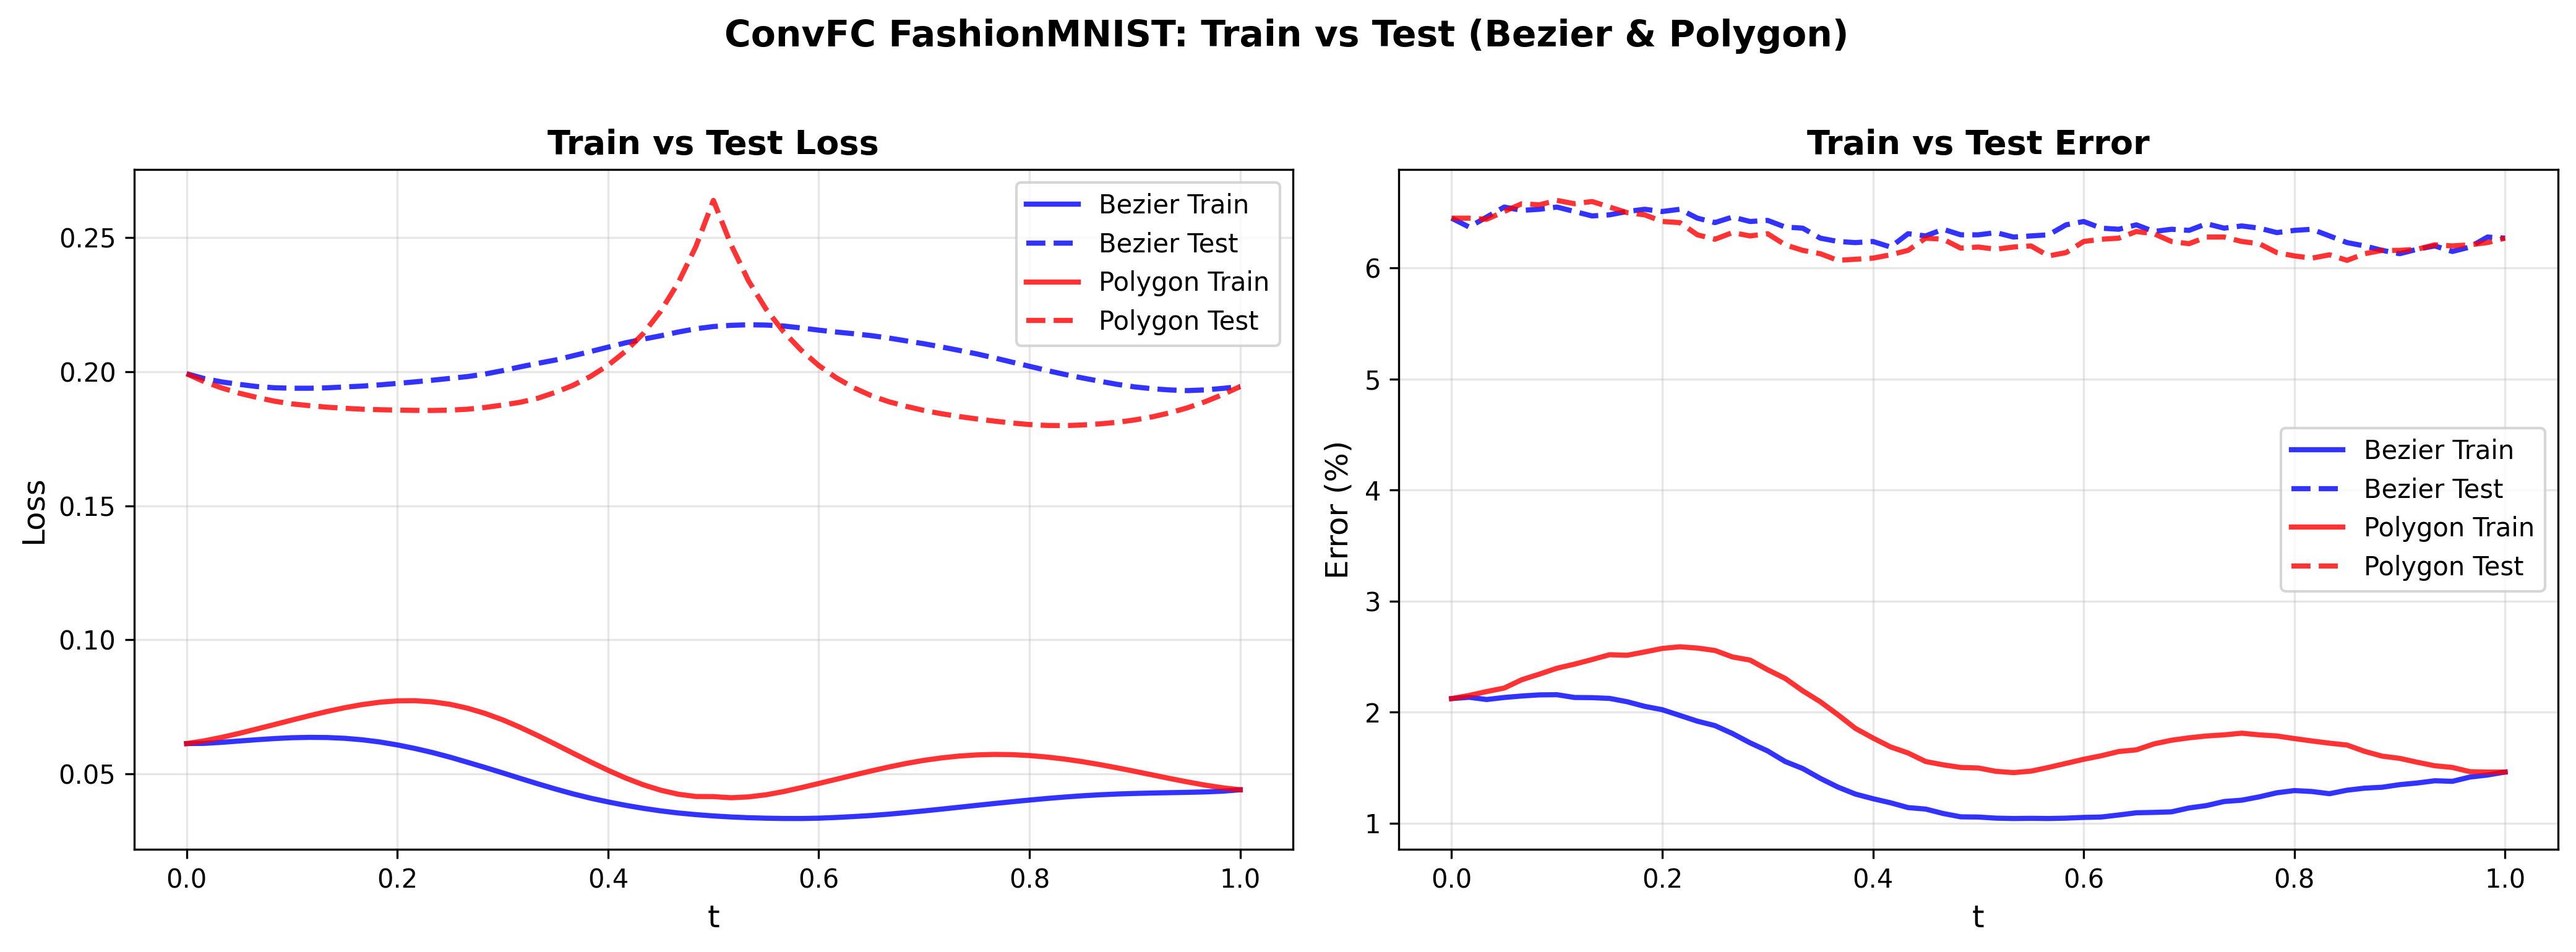
\includegraphics[width=0.95\linewidth]{../draft_3/convfc.png}
    \caption{Architectures used in experiments: VGG16 and ConvFC.}
    \label{fig:architectures}
\end{figure}

\section{Methodology}

\subsection{Path-Finding Methods}

Three methods are used to find low-loss paths between trained models $w_0$ and $w_1$:

\begin{itemize}
    \item \textbf{B\'{e}zier curve (1-bend):} A quadratic B\'{e}zier curve $\theta(t) = (1-t)^2 w_0 + 2t(1-t)\theta_{\text{mid}} + t^2 w_1$, where $\theta_{\text{mid}}$ is a trainable middle point initialized at the midpoint $(w_0 + w_1)/2$.
    \item \textbf{Polygon chain:} A piecewise linear path with one trainable bend point, offering an unconstrained baseline.
    \item \textbf{Symmetry plane constrained polygon:} A polygon chain where the middle bend is projected onto the perpendicular bisector hyperplane between $w_0$ and $w_1$ after each gradient step: $\theta_{\text{new}} = \theta - \frac{(\theta - \mathbf{m}) \cdot \mathbf{n}}{\|\mathbf{n}\|^2} \mathbf{n}$, where $\mathbf{m} = (w_0 + w_1)/2$ and $\mathbf{n} = w_1 - w_0$.
\end{itemize}

\subsection{Evaluation Protocol}
\label{sec:evaluation-protocol}

All paths are evaluated at 61 uniformly spaced points $t \in [0, 1]$. At each point, batch normalization statistics are recalculated on the training set (without augmentation), and both training and test metrics are recorded. The primary connectivity metric is the \textbf{barrier height}:
\[
\text{Barrier Height} = \max_{t \in [0,1]} \text{Error}(t) - \frac{\text{Error}(0) + \text{Error}(1)}{2}.
\]

\section{Completed Experiments and Findings}

\subsection{Effect of L2 Regularization on Curve Training}

B\'{e}zier curves were trained between seed0--seed1 and seed0--mirror endpoint pairs, with and without L2 regularization ($\lambda = 5 \times 10^{-4}$).

\textbf{Results:} Both configurations successfully connected modes with low barriers. Without regularization, curves achieved near-zero training error (0.14\%) but exhibited larger test barriers, indicating overfitting of the path itself. With regularization, test generalization along the path improved at the cost of slightly higher training error. Multiple training runs with different random seeds produced consistent results, confirming that the observed connectivity patterns are robust properties of the loss landscape rather than artifacts of specific training trajectories.

\begin{figure}[H]
    \centering
    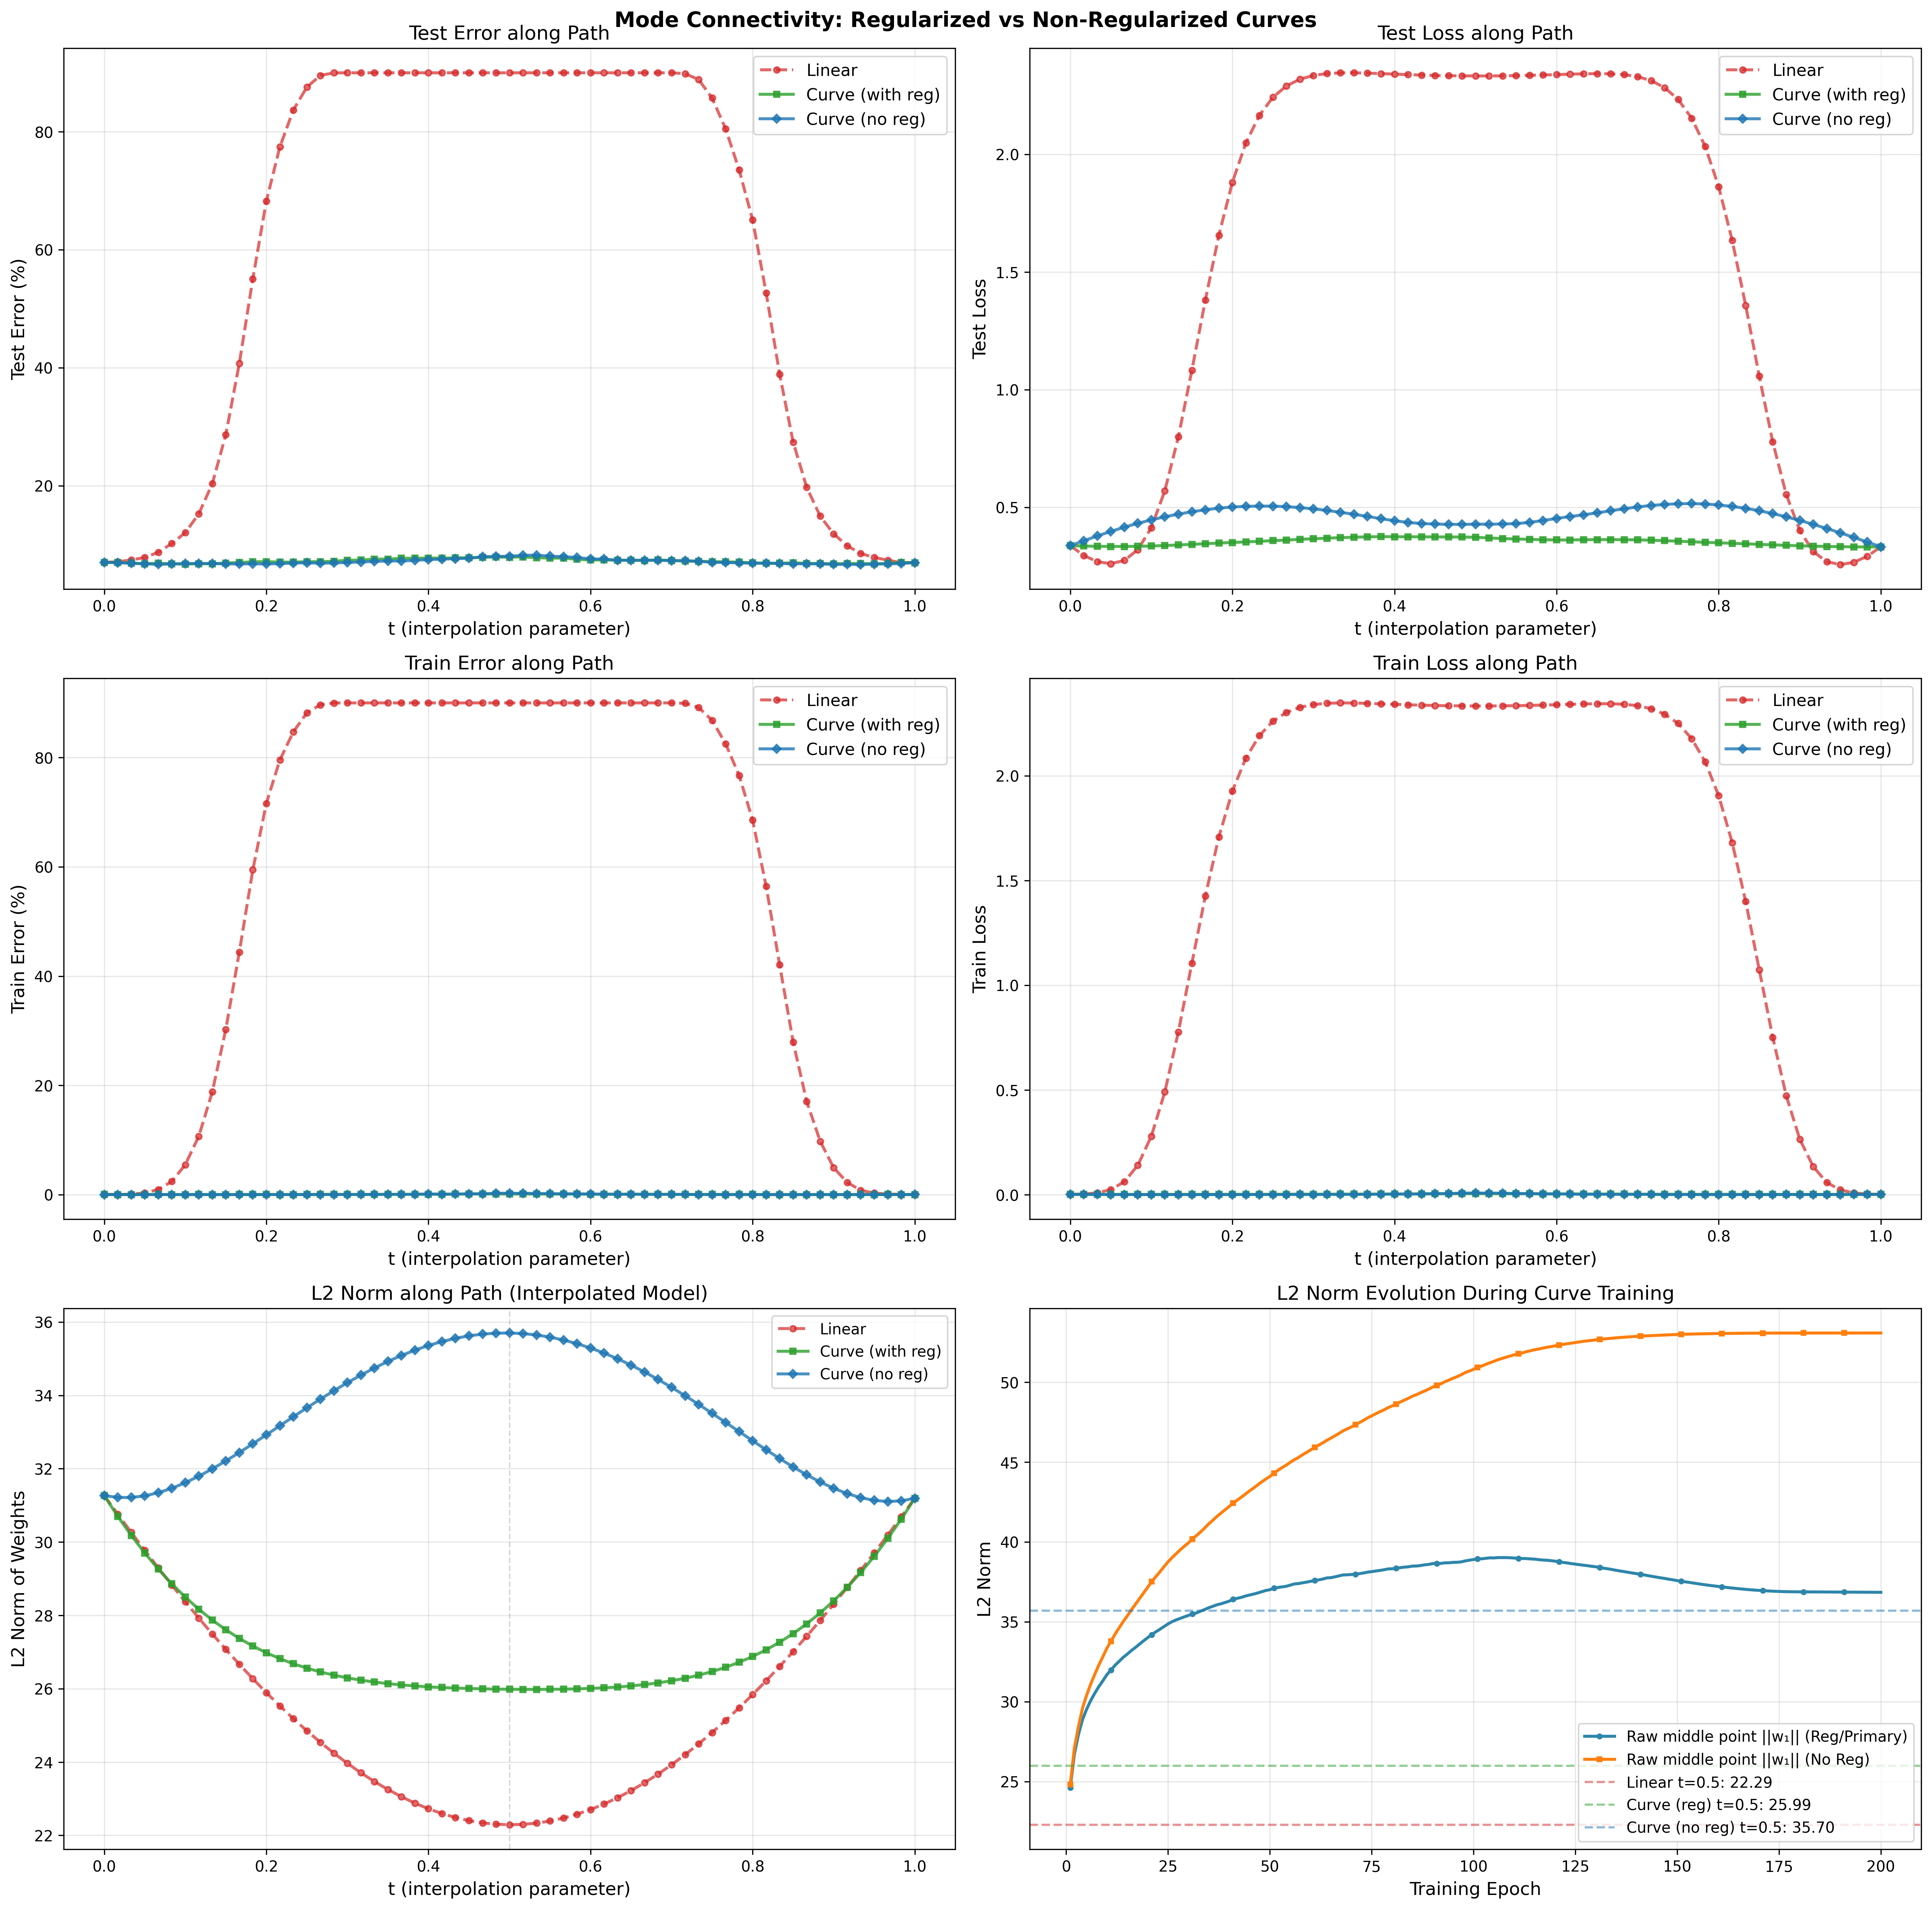
\includegraphics[width=0.95\linewidth]{../draft_1/lmc_reg_vs_noreg_comparison.png}
    \caption{Effect of L2 regularization on curve training (seed0--seed1 and seed0--mirror).}
    \label{fig:l2_reg_vs_noreg}
\end{figure}

\subsection{Neuron Permutation Experiments}

To investigate the effect of permutation invariance, 2-neuron swaps were performed in three different layers (early, middle, late) of VGG16. The L2 norm difference between the original and neuron-swapped interpolation paths was measured.

\textbf{Results:} Neuron permutations broke linear mode connectivity, with early layers exhibiting greater sensitivity than later layers. However, training B\'{e}zier curves between a mode and its permuted version successfully found low-loss paths within a few epochs, demonstrating that trainable curves can overcome permutation-induced barriers.

\begin{figure}[H]
    \centering
    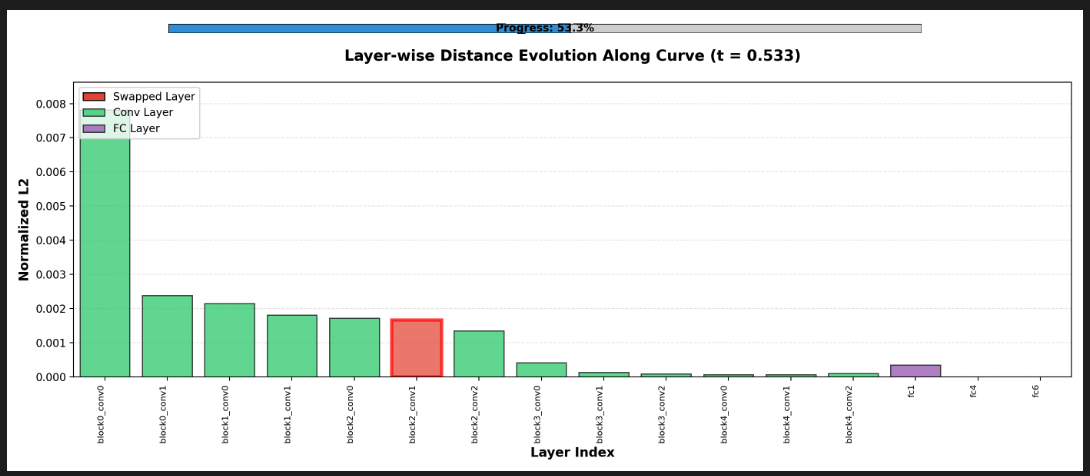
\includegraphics[width=0.9\linewidth]{../draft_1/sd.png}\\[0.5em]
    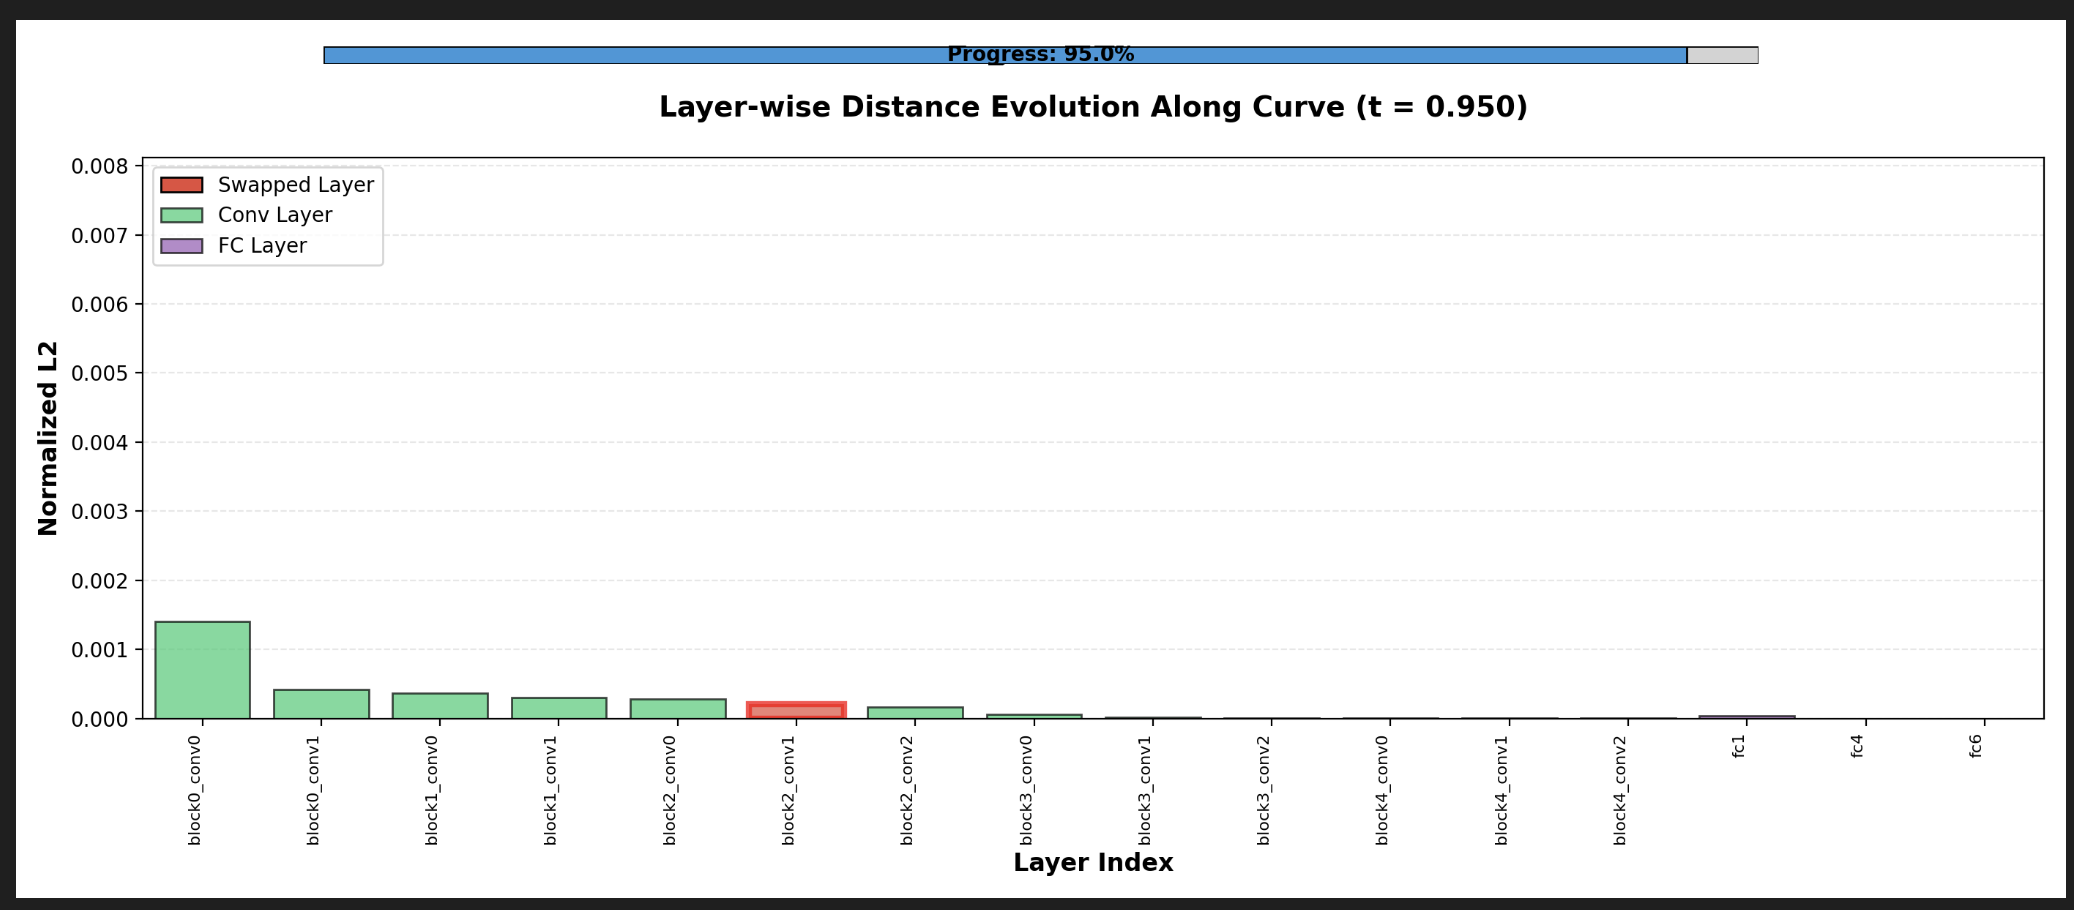
\includegraphics[width=0.9\linewidth]{../draft_1/neuron_swap_v2.png}
    \caption{Effect of neuron swaps on interpolation paths across layers.}
    \label{fig:neuron_swap}
\end{figure}

\begin{figure}[H]
    \centering
    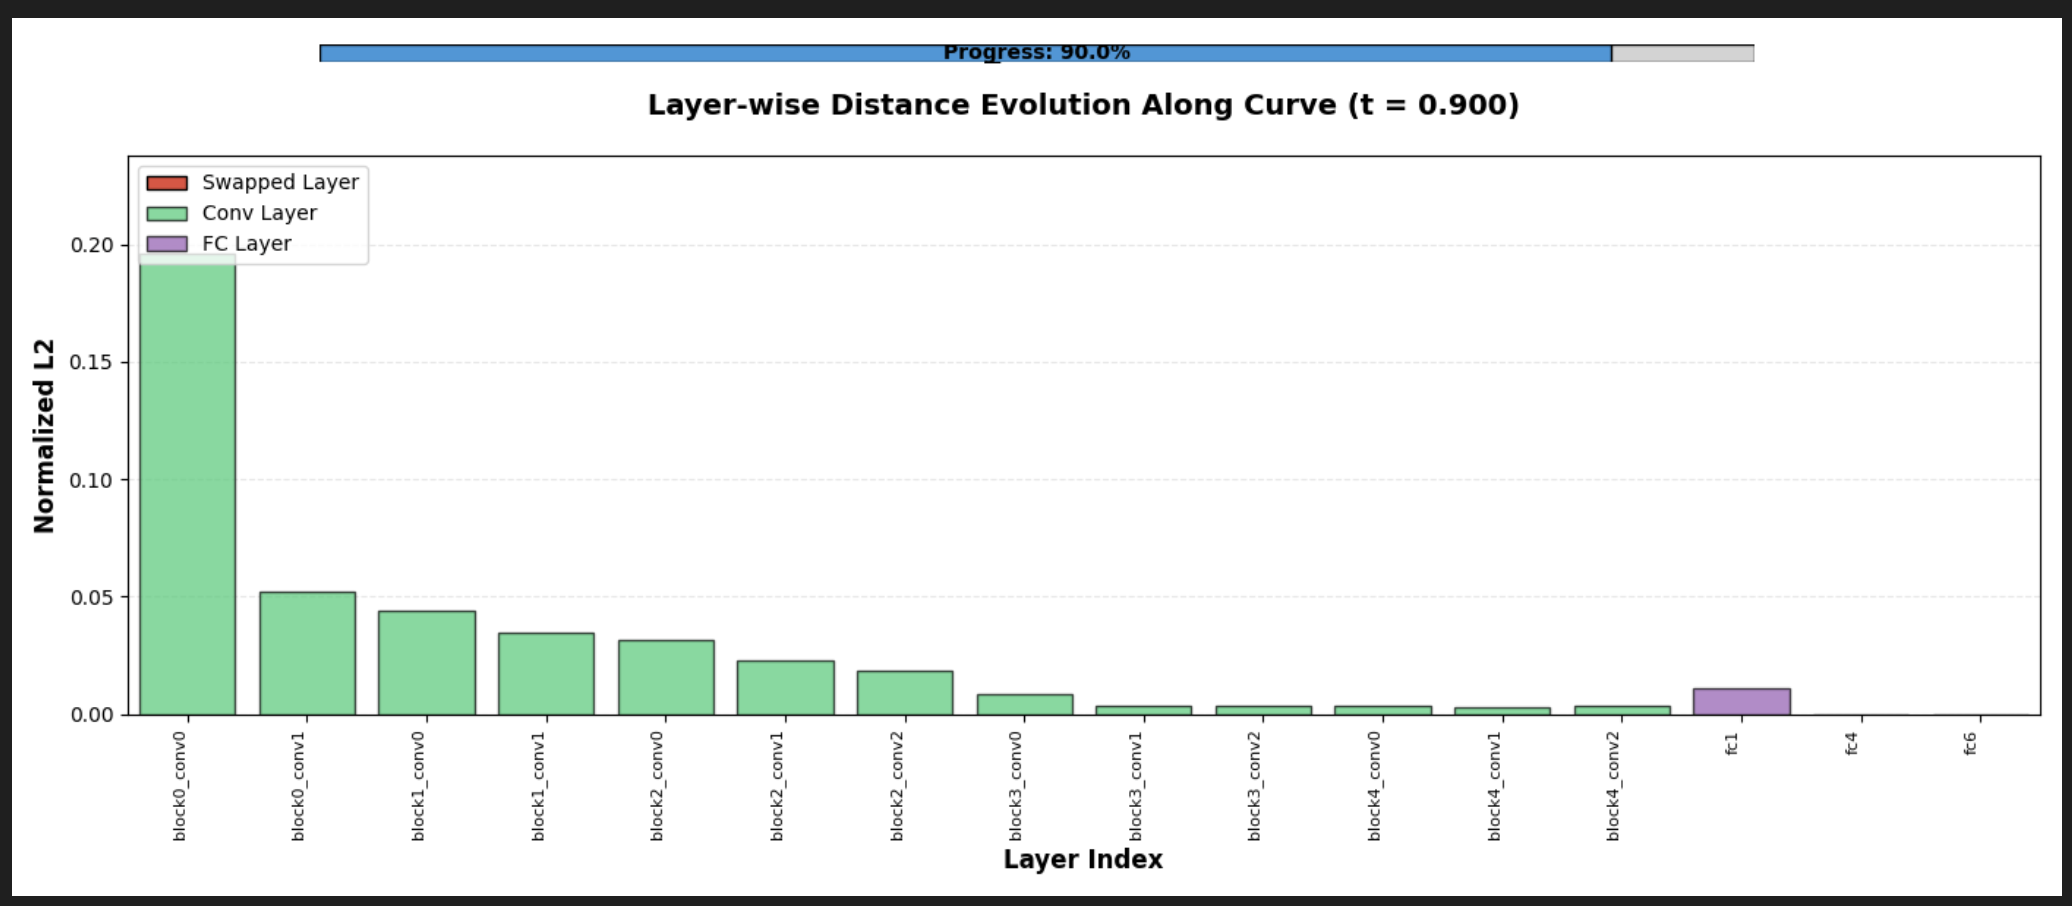
\includegraphics[width=0.9\linewidth]{../draft_1/layer_distance_measure.png}
    \caption{Layer distance along the curve between seed0 and seed1 (no permutation).}
    \label{fig:layer_distance}
\end{figure}

\textbf{Confirmation of prior work:} Our experiments showed identical 
connectivity behavior between seed0--seed1 (different initializations) 
and seed0--mirror (full permutation), which is consistent with the 
conjecture by Entezari et al.\ (2021) that ``different final networks 
[from different initializations] are [equivalent to] applying random 
permutations to the same SGD solution.''
\subsection{Hyperplane-Constrained Path Finding}

The perpendicular bisector (symmetry plane) between two endpoints $w_0$ and $w_1$ is a geometrically natural hyperplane: every point on it is equidistant from both endpoints. The original idea was to find a low-loss path from one endpoint to any point on this plane, and then mirror it to construct a full symmetric path between the two modes. To explore this, we constrained the middle bend of a polygon chain to lie on the symmetry plane by projecting it after each gradient step. The constraint was verified using the normalized distance $d_{\text{norm}} = \frac{|(\theta - \mathbf{m}) \cdot \mathbf{n}|}{\|\mathbf{n}\| \cdot \sqrt{N}}$, achieving machine-precision satisfaction ($d_{\text{norm}} \approx 7.2 \times 10^{-8}$).

The constrained optimization found low-loss paths with no deterioration in quality compared to unconstrained optimization:

\begin{table}[H]
    \centering
    \caption{Test Error and Barrier Height Comparison (seed0--mirror, VGG16/CIFAR-10)}
    \label{tab:performance}
    \begin{tabular}{l c c}
        \toprule
        \textbf{Method} & \textbf{Max Test Error (\%)} & \textbf{Barrier Height (\%)} \\
        \midrule
        Polygon Chain (unconstrained) & $9.21$ & $2.22$ \\
        Symmetry Plane (constrained) & $8.81$ & $1.82$ \\
        B\'{e}zier Curve & $9.37$ & $2.38$ \\
        \bottomrule
    \end{tabular}
\end{table}

\begin{figure}[H]
    \centering
    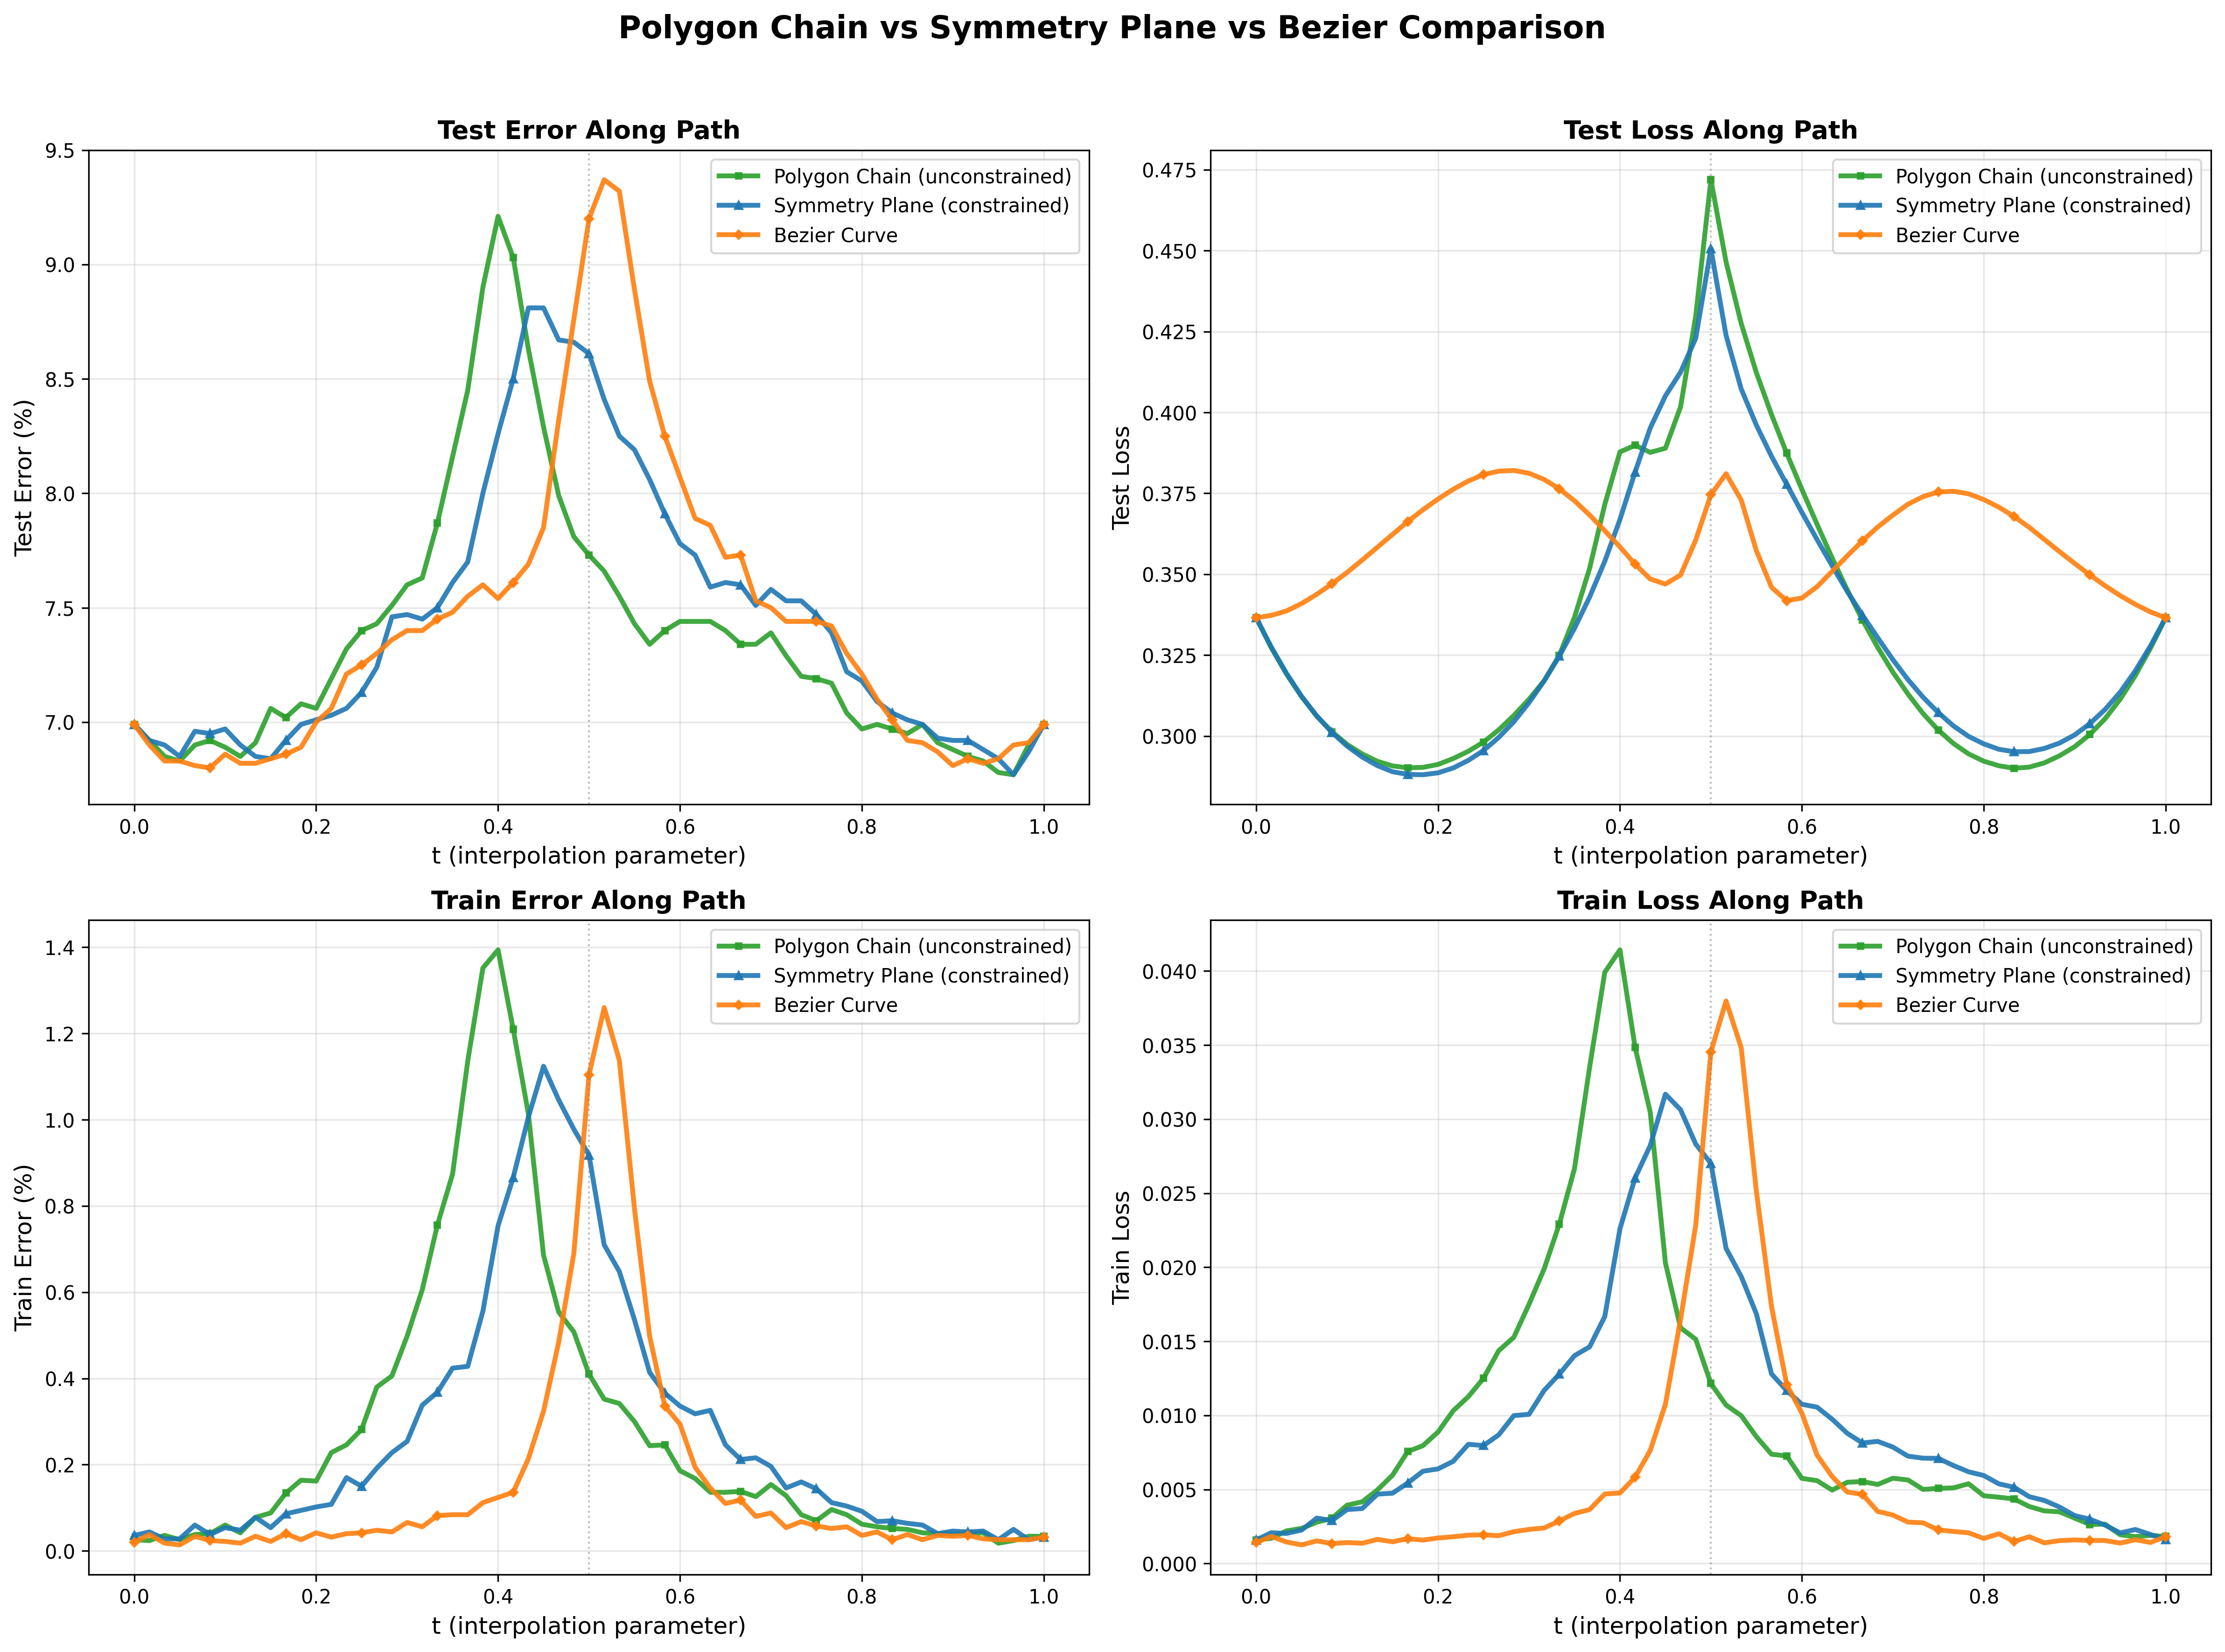
\includegraphics[width=0.9\linewidth]{../draft_1/polygon_vs_symmetry.png}
    \caption{Comparison of low-loss path finding methods (polygon chain, symmetry plane, B\'{e}zier).}
    \label{fig:polygon_vs_symmetry}
\end{figure}

The optimized middle bend moved approximately 64\% of the endpoint separation distance from the geometric midpoint, with this movement being primarily tangential to the symmetry plane. Observing that the constraint did not degrade connectivity raised a natural question: is the symmetry plane geometrically special, or would any hyperplane work equally well?

To answer this, we tested two additional hyperplane types:

\begin{table}[H]
\centering
\caption{Hyperplane Constraint Configurations}
\begin{tabular}{lll}
\toprule
\textbf{Plane Type} & \textbf{Anchor Point} & \textbf{Normal Vector} \\
\midrule
Symmetry Plane & Midpoint $(w_0+w_1)/2$ & $w_1-w_0$ \\
Random Plane (Midpoint) & Midpoint $(w_0+w_1)/2$ & Random unit vector \\
Random Plane (Random) & Random $\alpha w_0+(1-\alpha)w_1$ & Random unit vector \\
\bottomrule
\end{tabular}
\end{table}

\textbf{Results:} All three hyperplane constraints yielded nearly identical connectivity performance. Test error curves, training loss, and barrier heights showed no meaningful differences. The unconstrained polygon chain also produced similar results.

\begin{figure}[H]
    \centering
    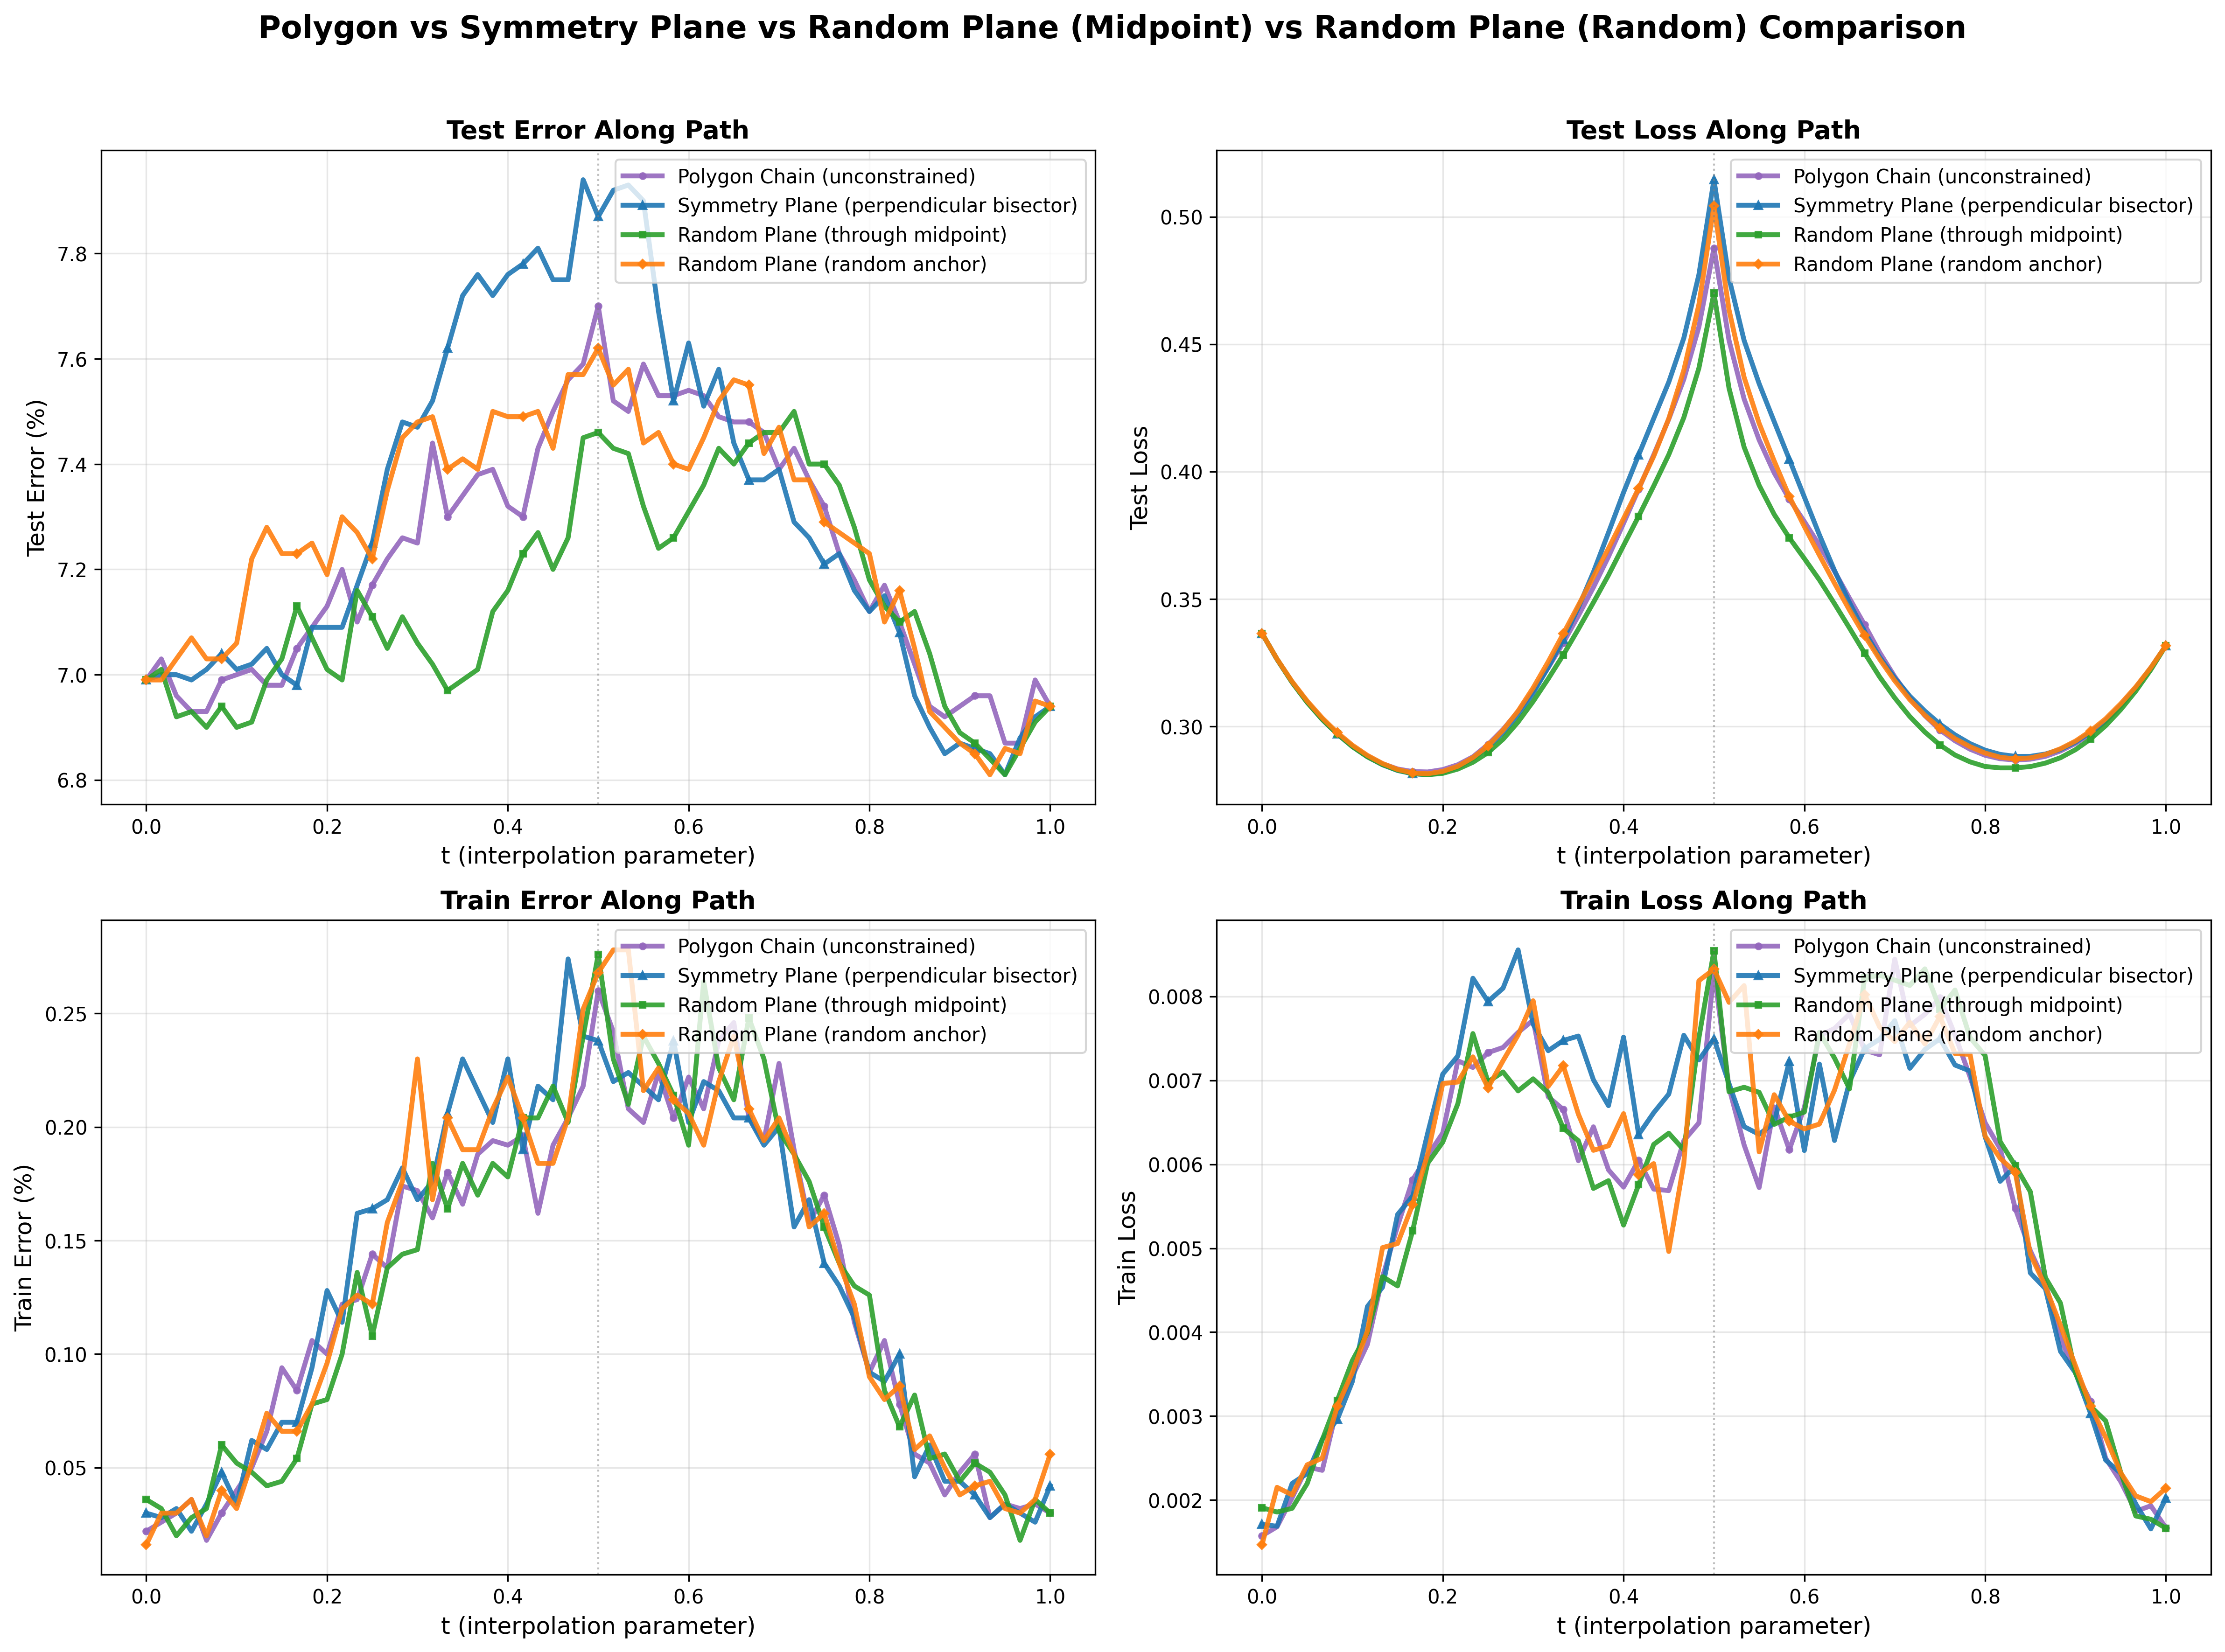
\includegraphics[width=0.85\linewidth]{../draft_2/random_planes_comp.png}
    \caption{Random hyperplane constraints yield similar connectivity performance.}
    \label{fig:random_planes}
\end{figure}

\textbf{Interpretation:} Each hyperplane constraint removes exactly one direction from $\sim$15 million dimensional parameter space ($N$ to $N-1$ dimensions). This is an extremely weak constraint with negligible impact on the optimization landscape. Low-loss paths exist within any $(N-1)$-dimensional hyperplane, regardless of orientation or anchor point. The symmetry plane maintained connectivity not because of special geometric properties of the perpendicular bisector, but because any single-direction constraint is effectively non-restrictive in such high-dimensional spaces.

\subsection{Initialization Strategy Robustness}

Three initialization strategies for the trainable middle bend of B\'{e}zier curves were compared (without regularization):

\begin{itemize}
    \item \textbf{Biased linear:} $\theta_{\text{init}} = \alpha w_0 + (1-\alpha) w_1$ with $\alpha \in \{0.75, 0.9\}$
    \item \textbf{Perturbed midpoint:} $\theta_{\text{init}} = 0.5(w_0 + w_1) + \epsilon$, $\epsilon \sim \mathcal{N}(0, \sigma^2 I)$
    \item \textbf{Sphere-constrained:} Midpoint with noise, projected onto a sphere
\end{itemize}

\textbf{Results:} All strategies converged to low-loss paths, though barrier height increased with distance from the midpoint. Without regularization, the trained bend point remained at its initialized distance from the origin ($\sim$320 vs.\ $\sim$40 for regularized training), as there was no incentive to reduce the L2 norm.

\begin{figure}[H]
    \centering
    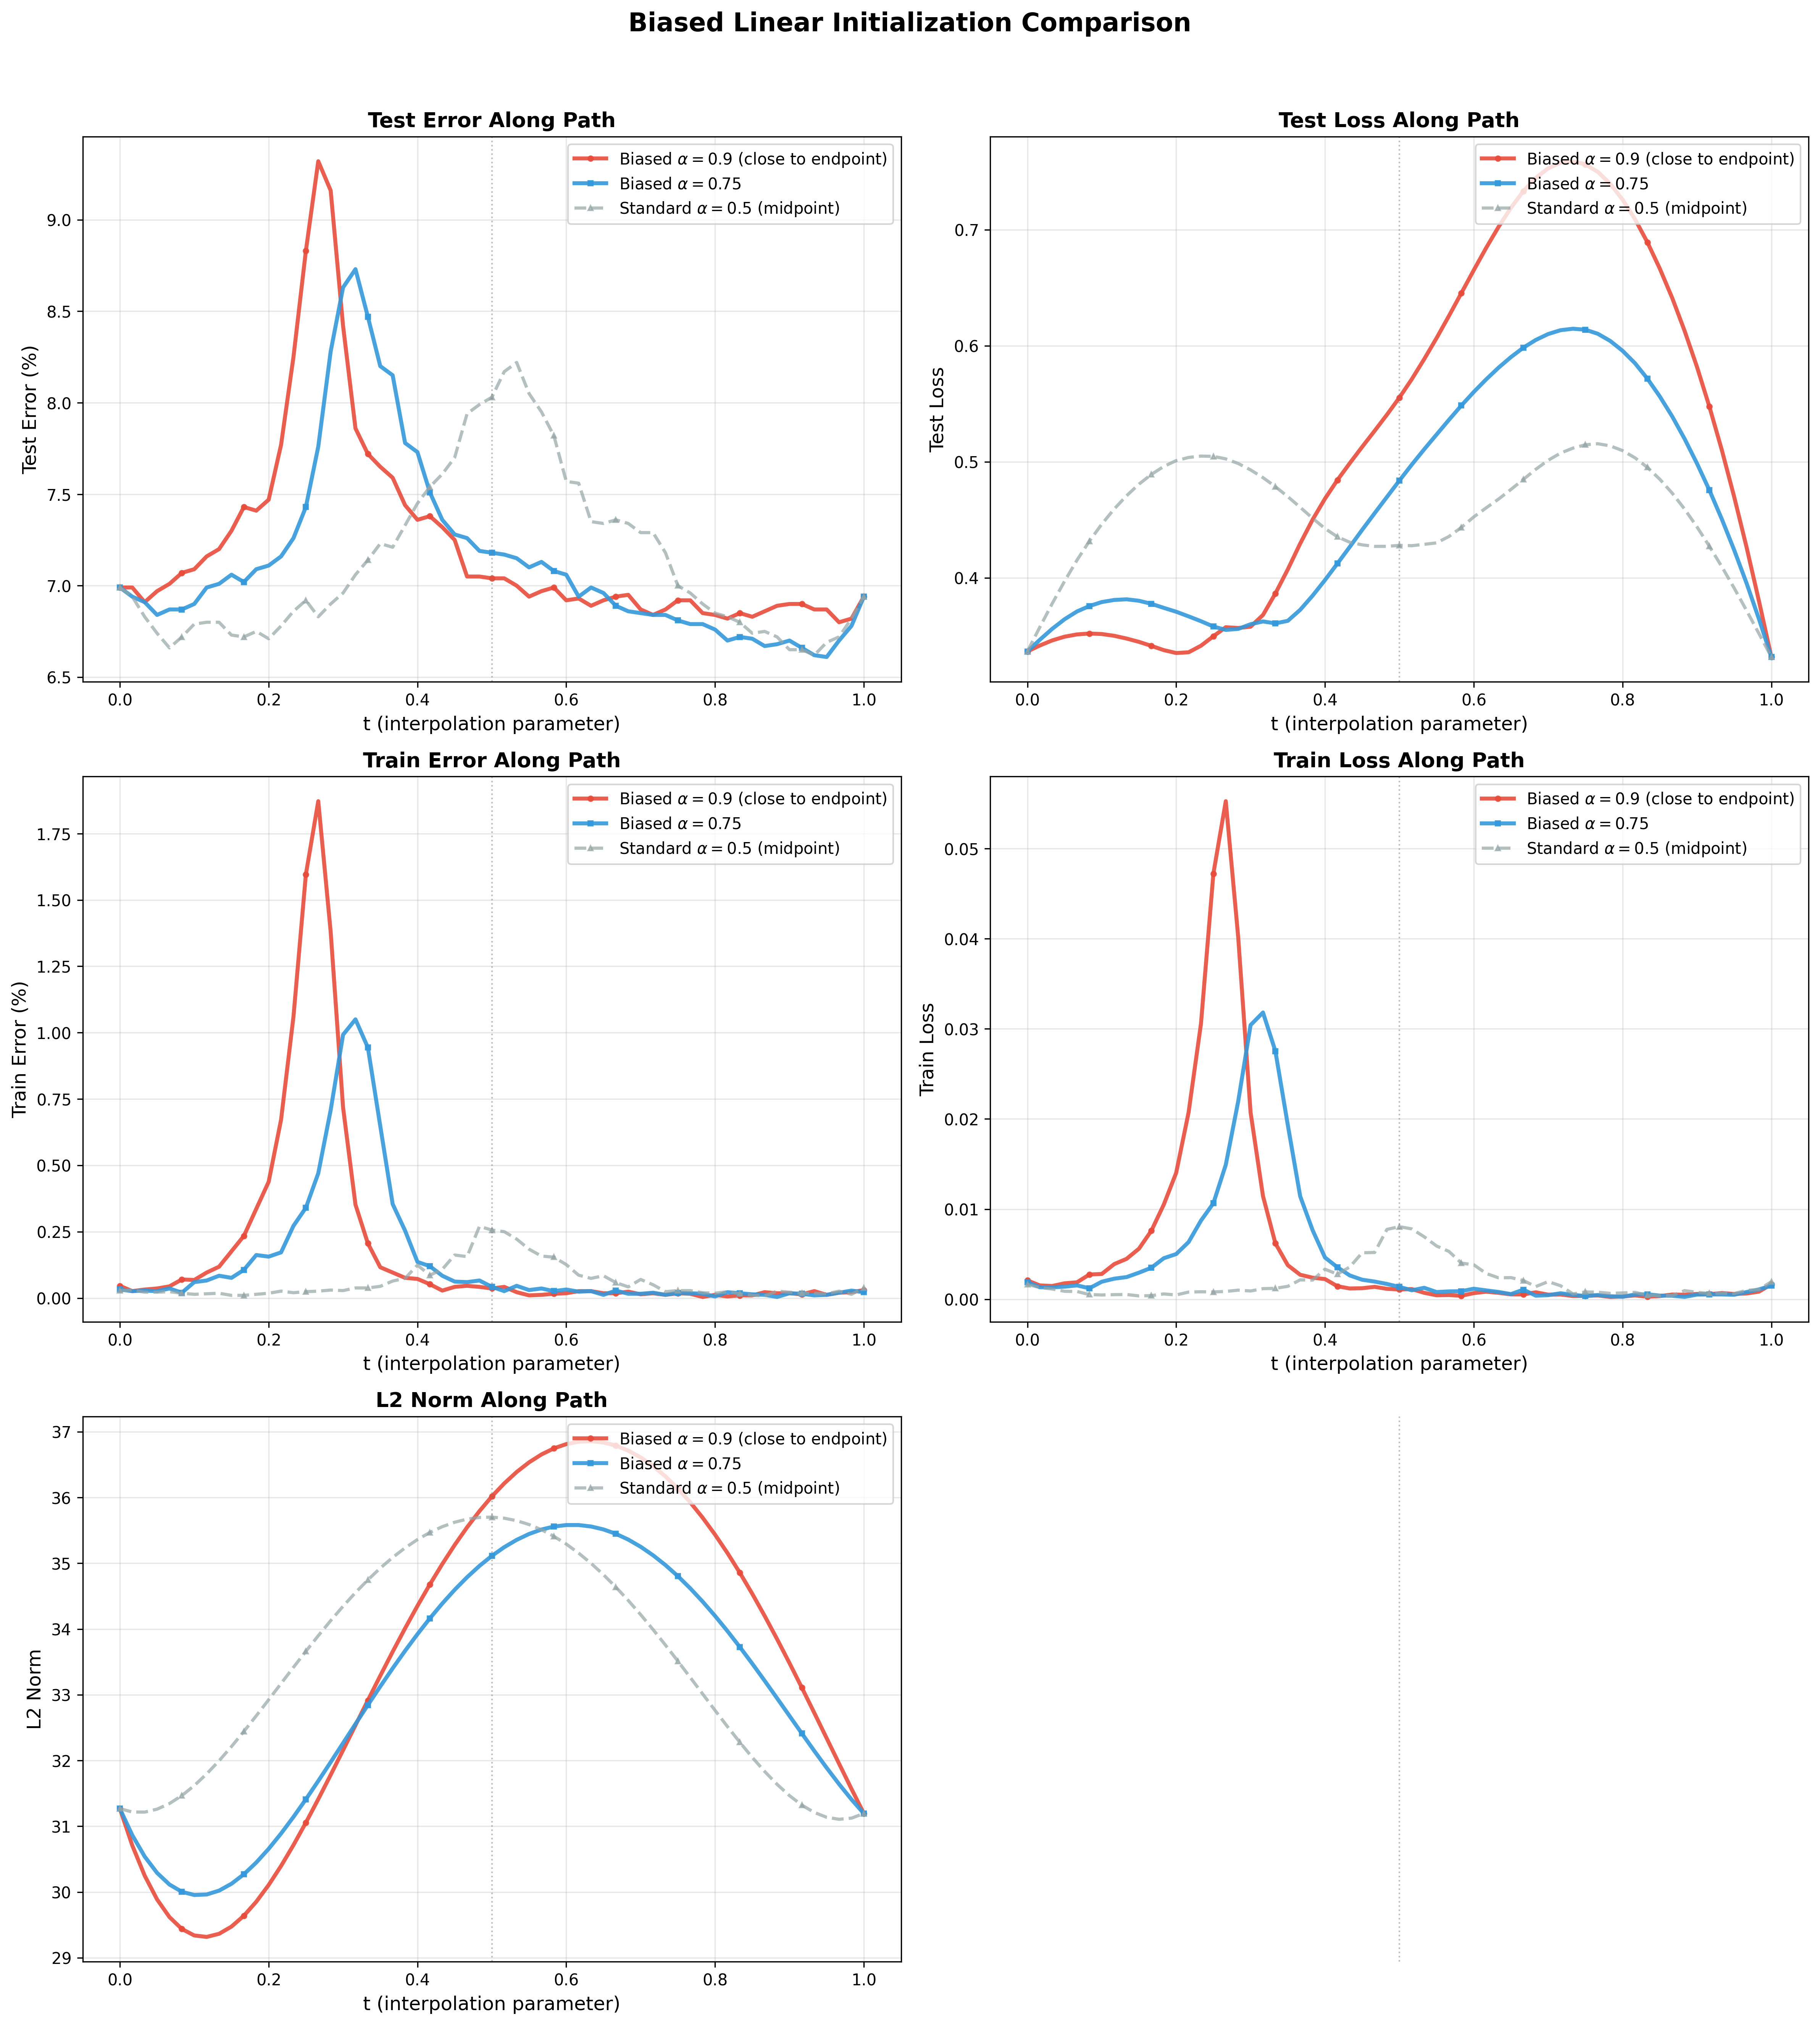
\includegraphics[width=0.95\linewidth]{../draft_2/init_comparison.png}
    \caption{Initialization strategies for the B\'{e}zier middle bend (biased linear vs.\ midpoint).}
    \label{fig:init_comparison}
\end{figure}

\begin{figure}[H]
    \centering
    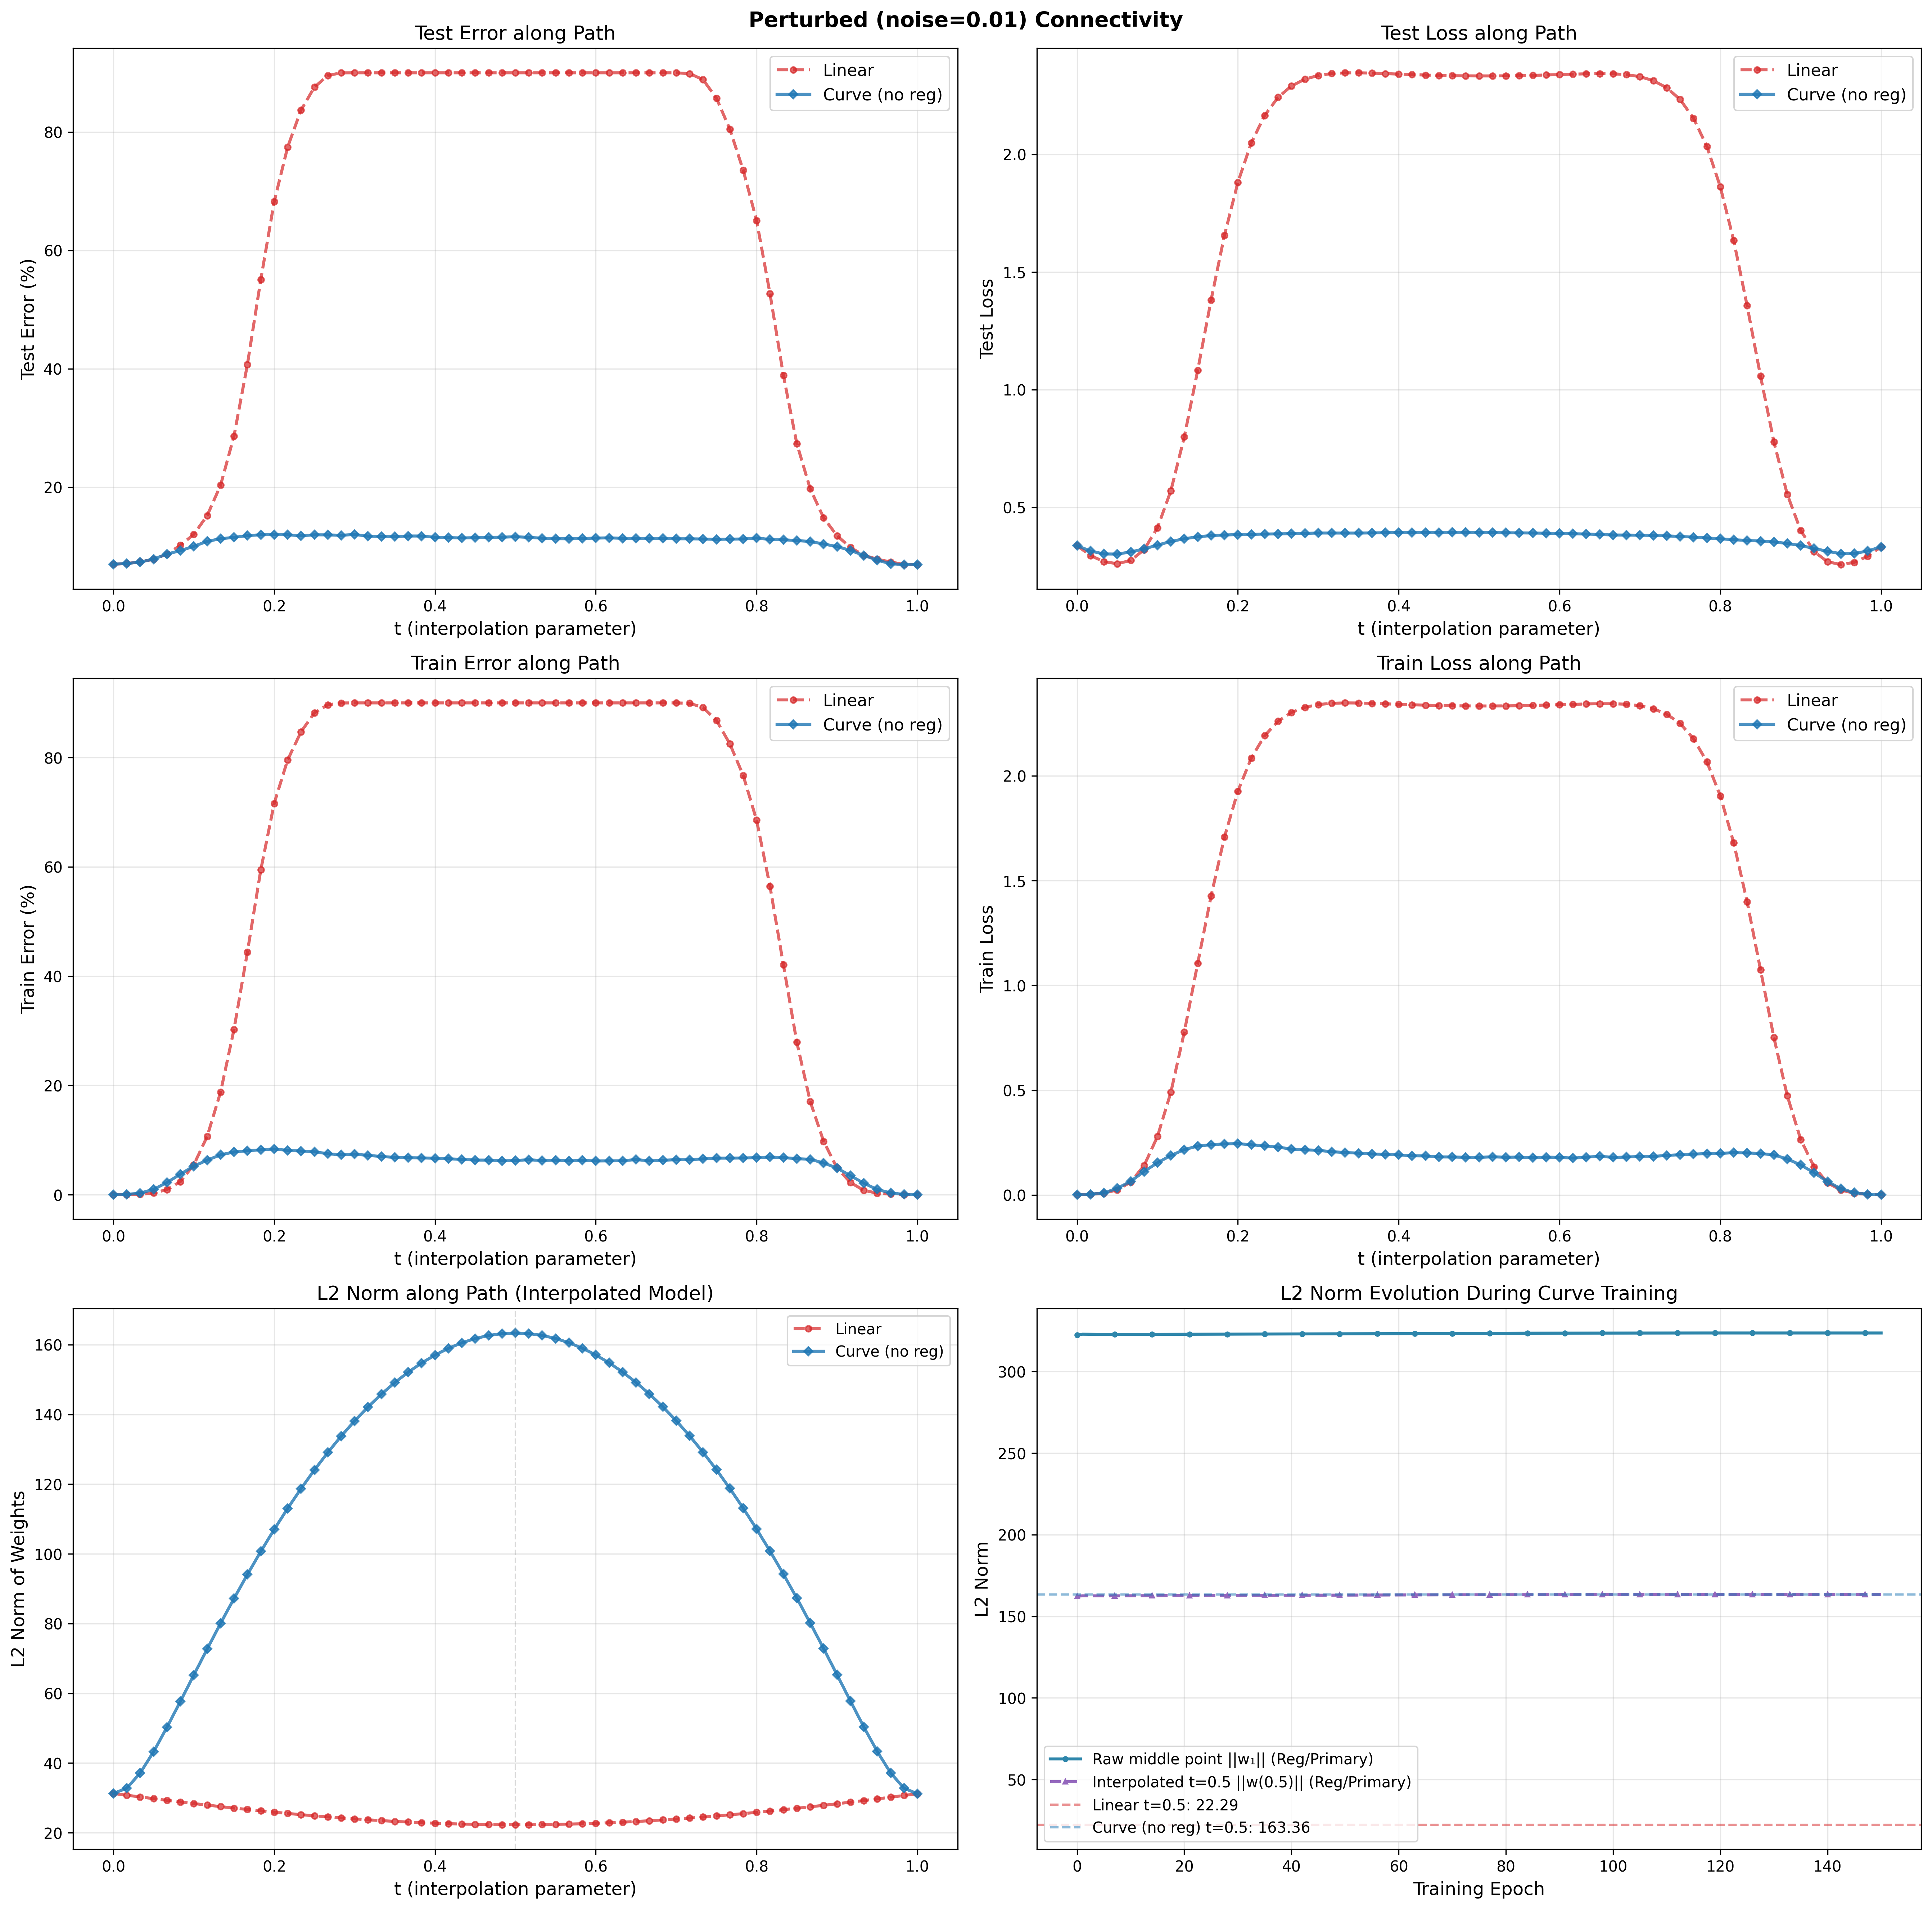
\includegraphics[width=0.95\linewidth]{../draft_2/perturbed.png}
    \caption{Perturbed midpoint initialization and resulting path behavior.}
    \label{fig:perturbed_init}
\end{figure}

\textbf{Interpretation:} The robustness to initialization indicates that the mode connectivity optimization problem has favorable geometric properties. Low-loss paths between modes are abundant rather than rare, and the optimization landscape does not exhibit narrow basins or strong dependence on initial positioning.

\subsection{Cross-Architecture Validation: ConvFC on Fashion-MNIST}

To validate generalizability, the same connectivity experiments were conducted using a ConvFC architecture on Fashion-MNIST. Results were qualitatively similar to VGG16 on CIFAR-10, confirming that mode connectivity phenomena generalize across model architectures and datasets.

\textbf{Notable differences:} The L2 norm along the trained curve path exhibited asymmetry around $t=0.5$, unlike the more symmetric behavior observed in VGG16, but that phenomenon can be explained by one mode exhibiting slightly better performance than the other. Despite this, the linear interpolation barrier remained symmetric. Barriers were visibly thinner than in VGG16/CIFAR-10.

\begin{figure}[H]
    \centering
    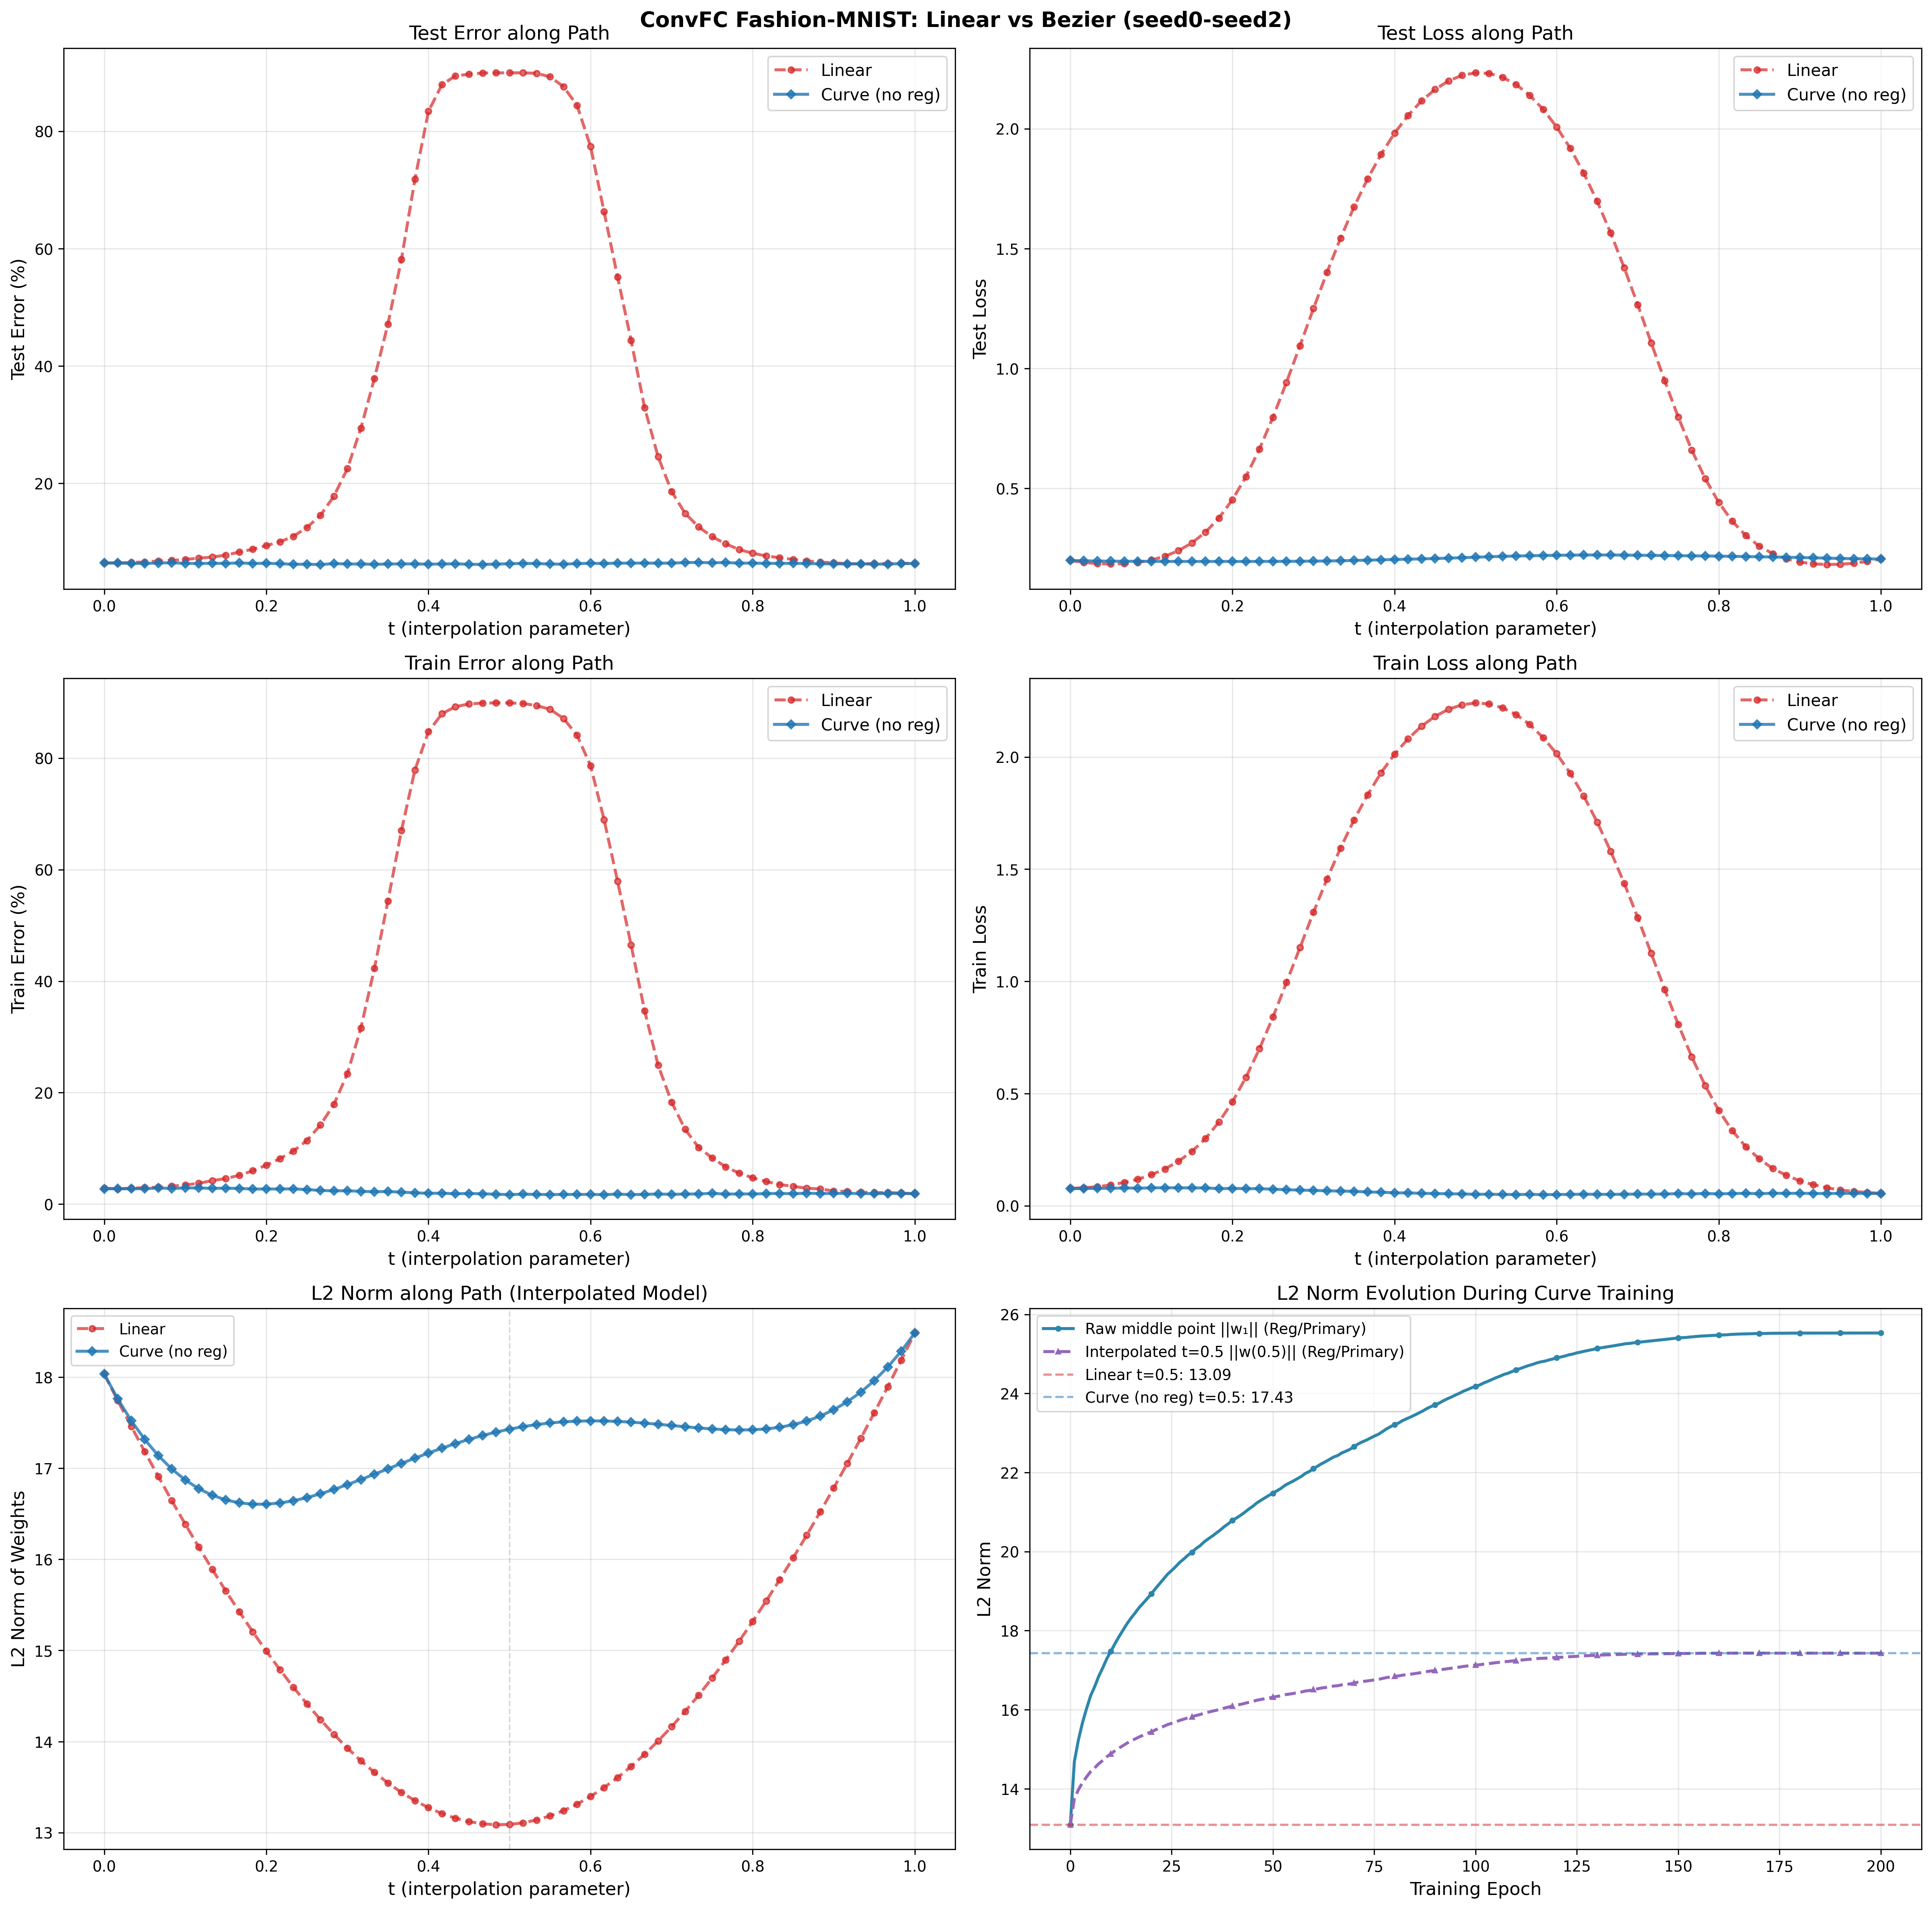
\includegraphics[width=0.9\linewidth]{../draft_2/convfc_example.png}
    \caption{ConvFC on Fashion-MNIST: example low-loss path and barrier profile.}
    \label{fig:convfc_example}
\end{figure}

\begin{figure}[H]
    \centering
    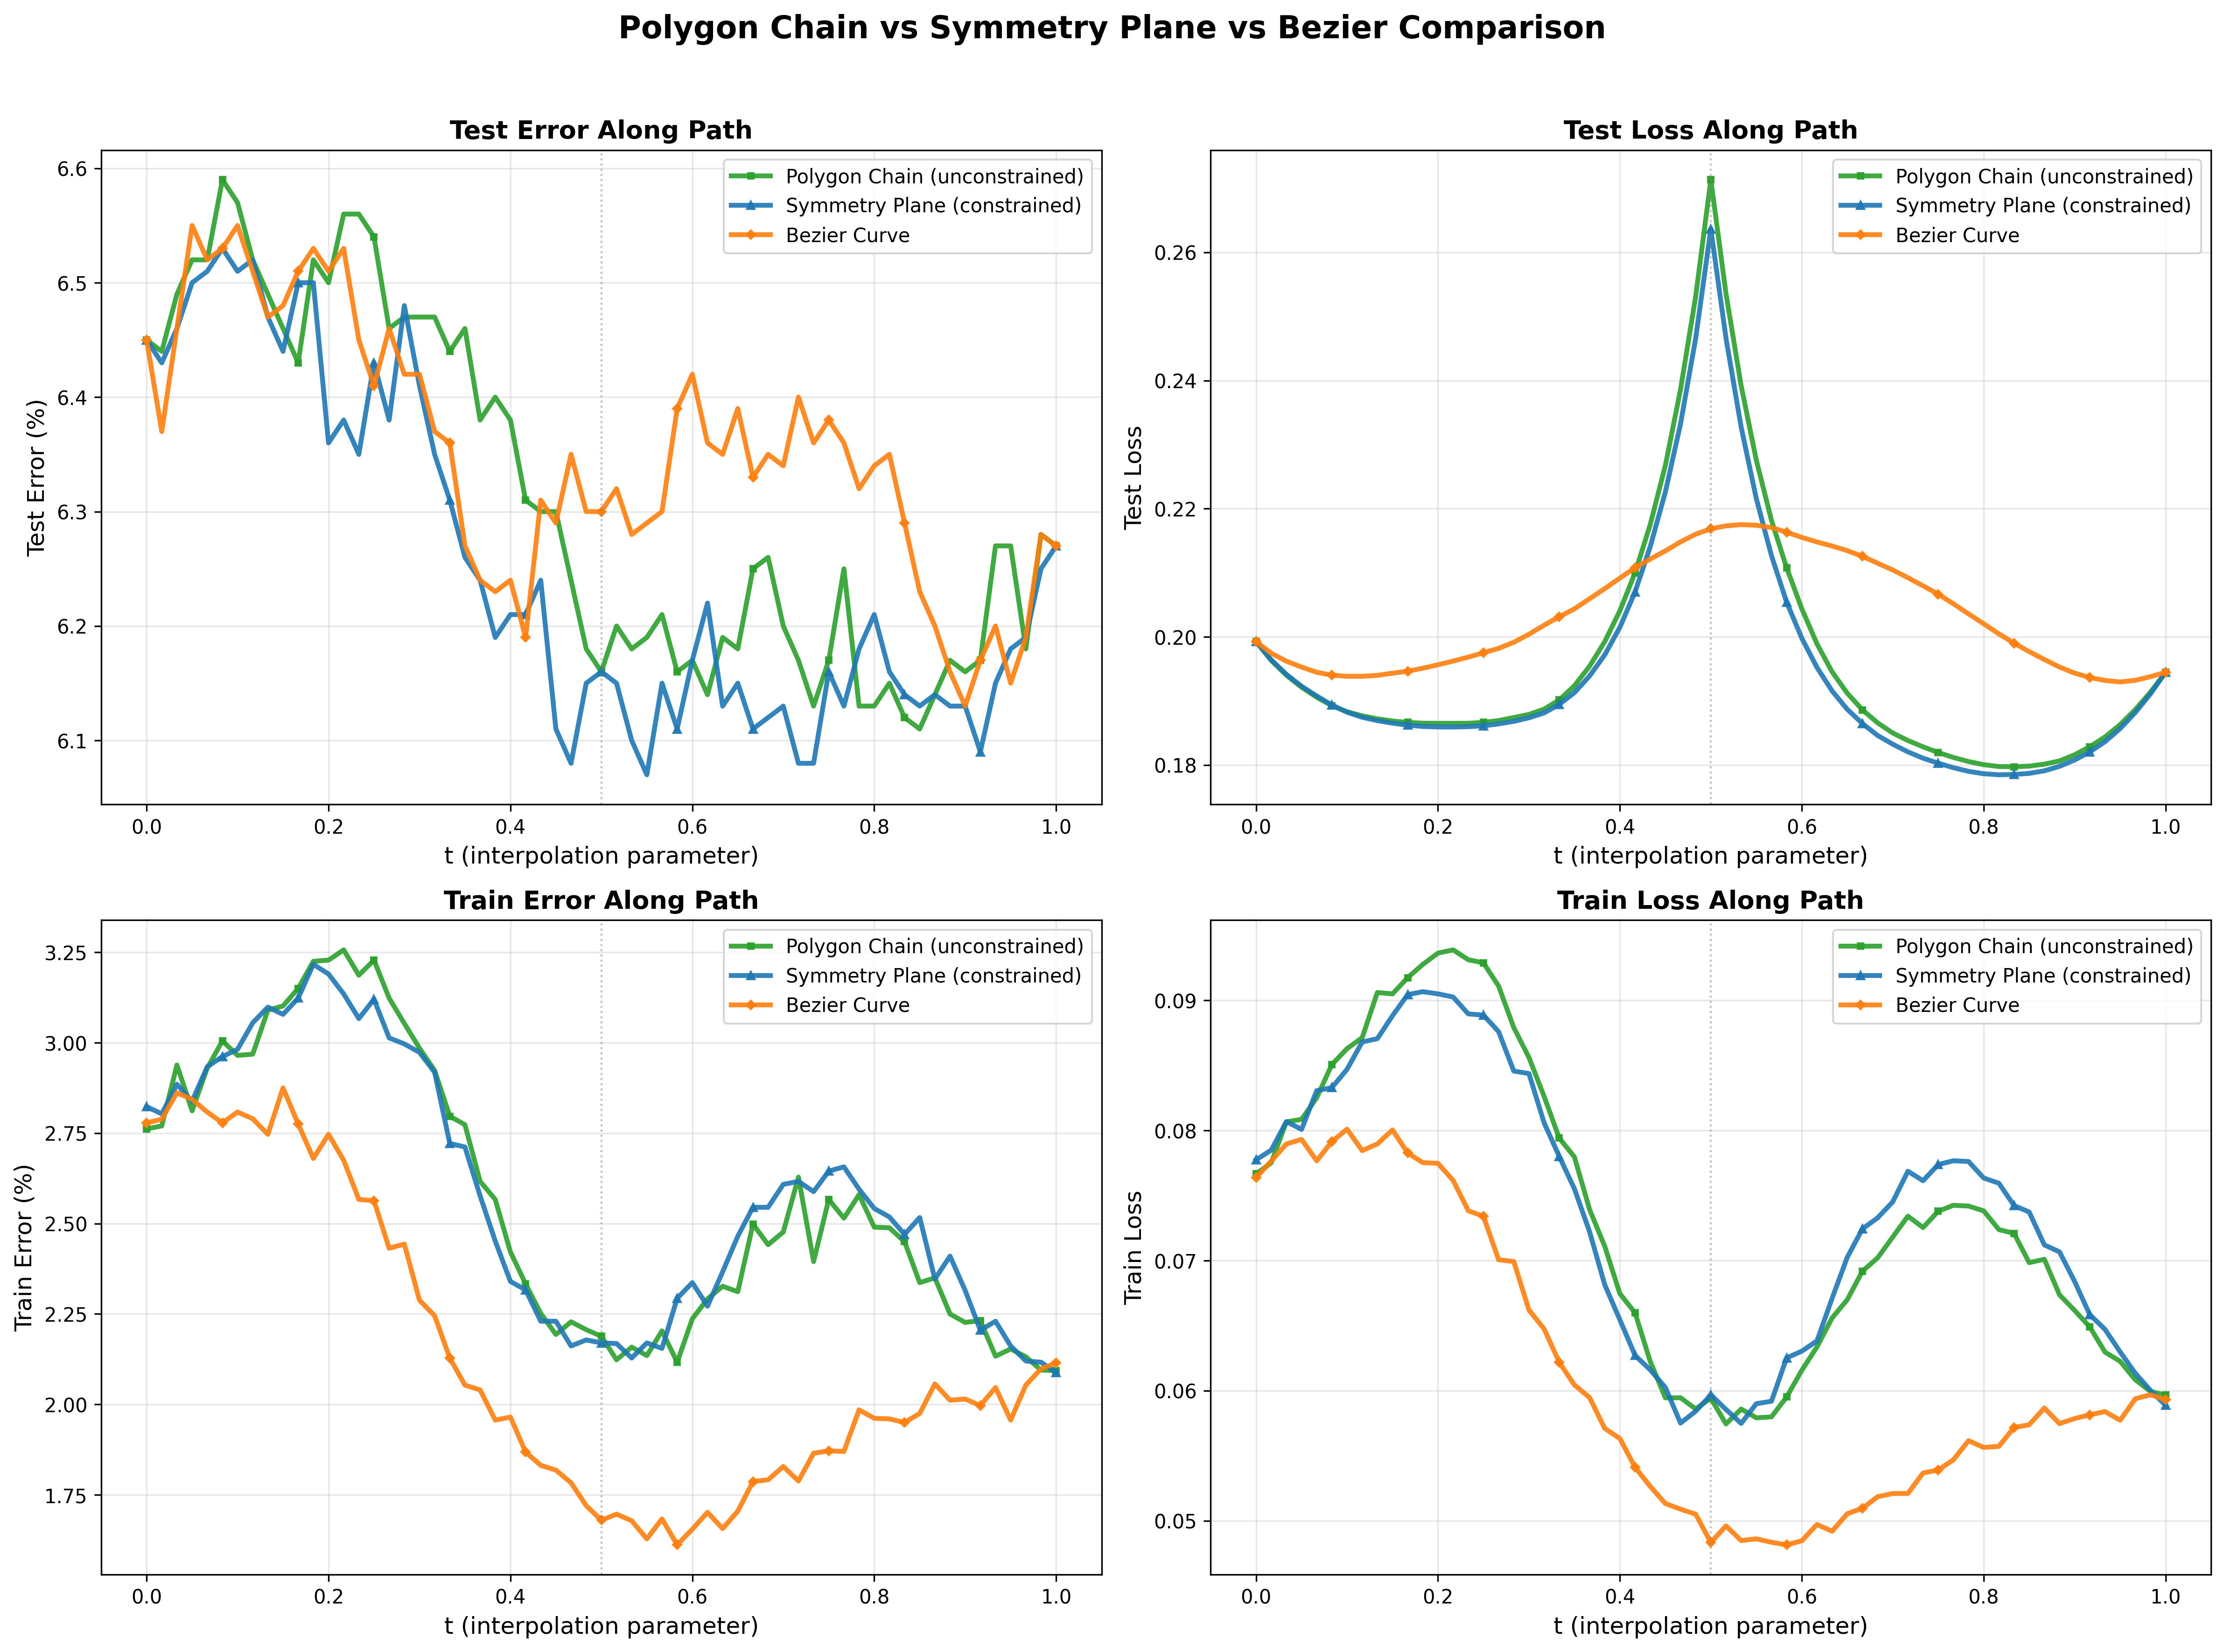
\includegraphics[width=0.8\linewidth]{../draft_2/seed0seed1curve_comparison.png}
    \caption{Seed0--seed1 low-loss path finding methods comparison.}
    \label{fig:seed0seed1_comparison}
\end{figure}

\subsection{Evaluation Methodology Fixes and Loss-Curve Diagnostics}

During verification, we identified that random data augmentations (horizontal flips and random crops) were being applied while recomputing batch normalization statistics on the training split. This introduced artificial noise in the evaluation curves and slight inconsistencies at the endpoints across path-finding methods. After disabling augmentations for evaluation, loss curves became smooth and endpoint metrics aligned as expected.

\begin{figure}[H]
    \centering
    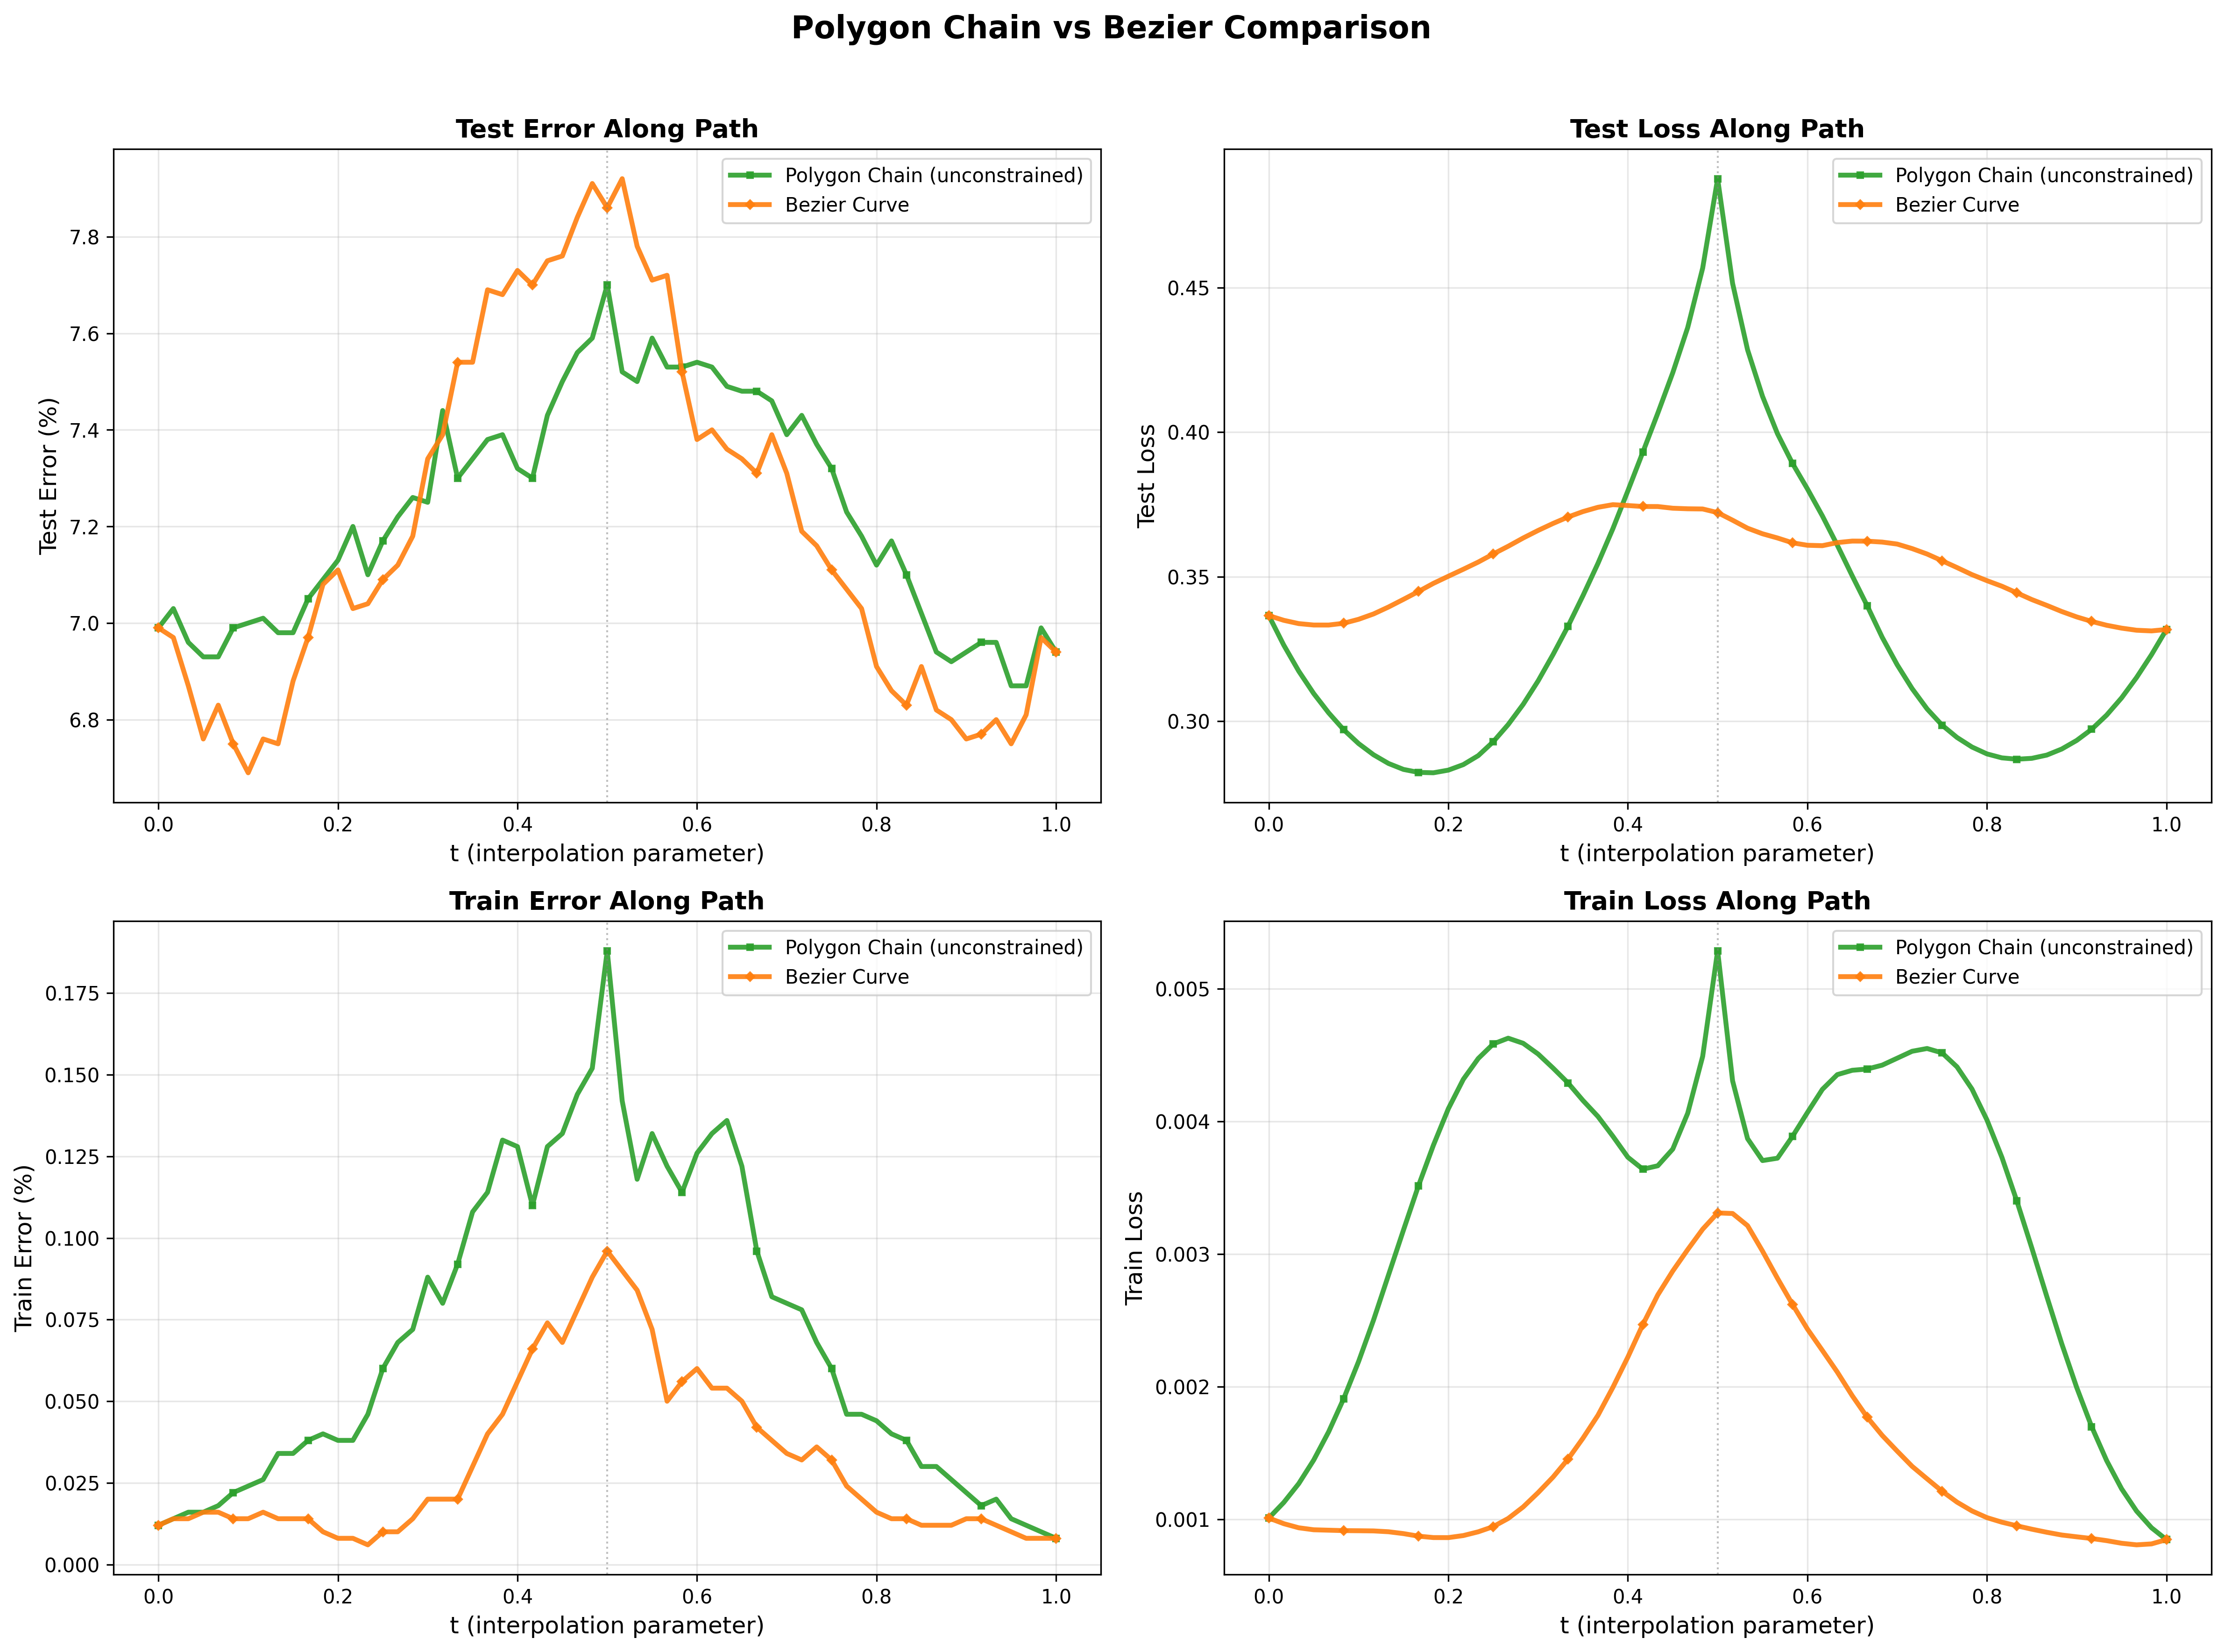
\includegraphics[width=0.95\linewidth]{../draft_3/example.png}\\[0.5em]
    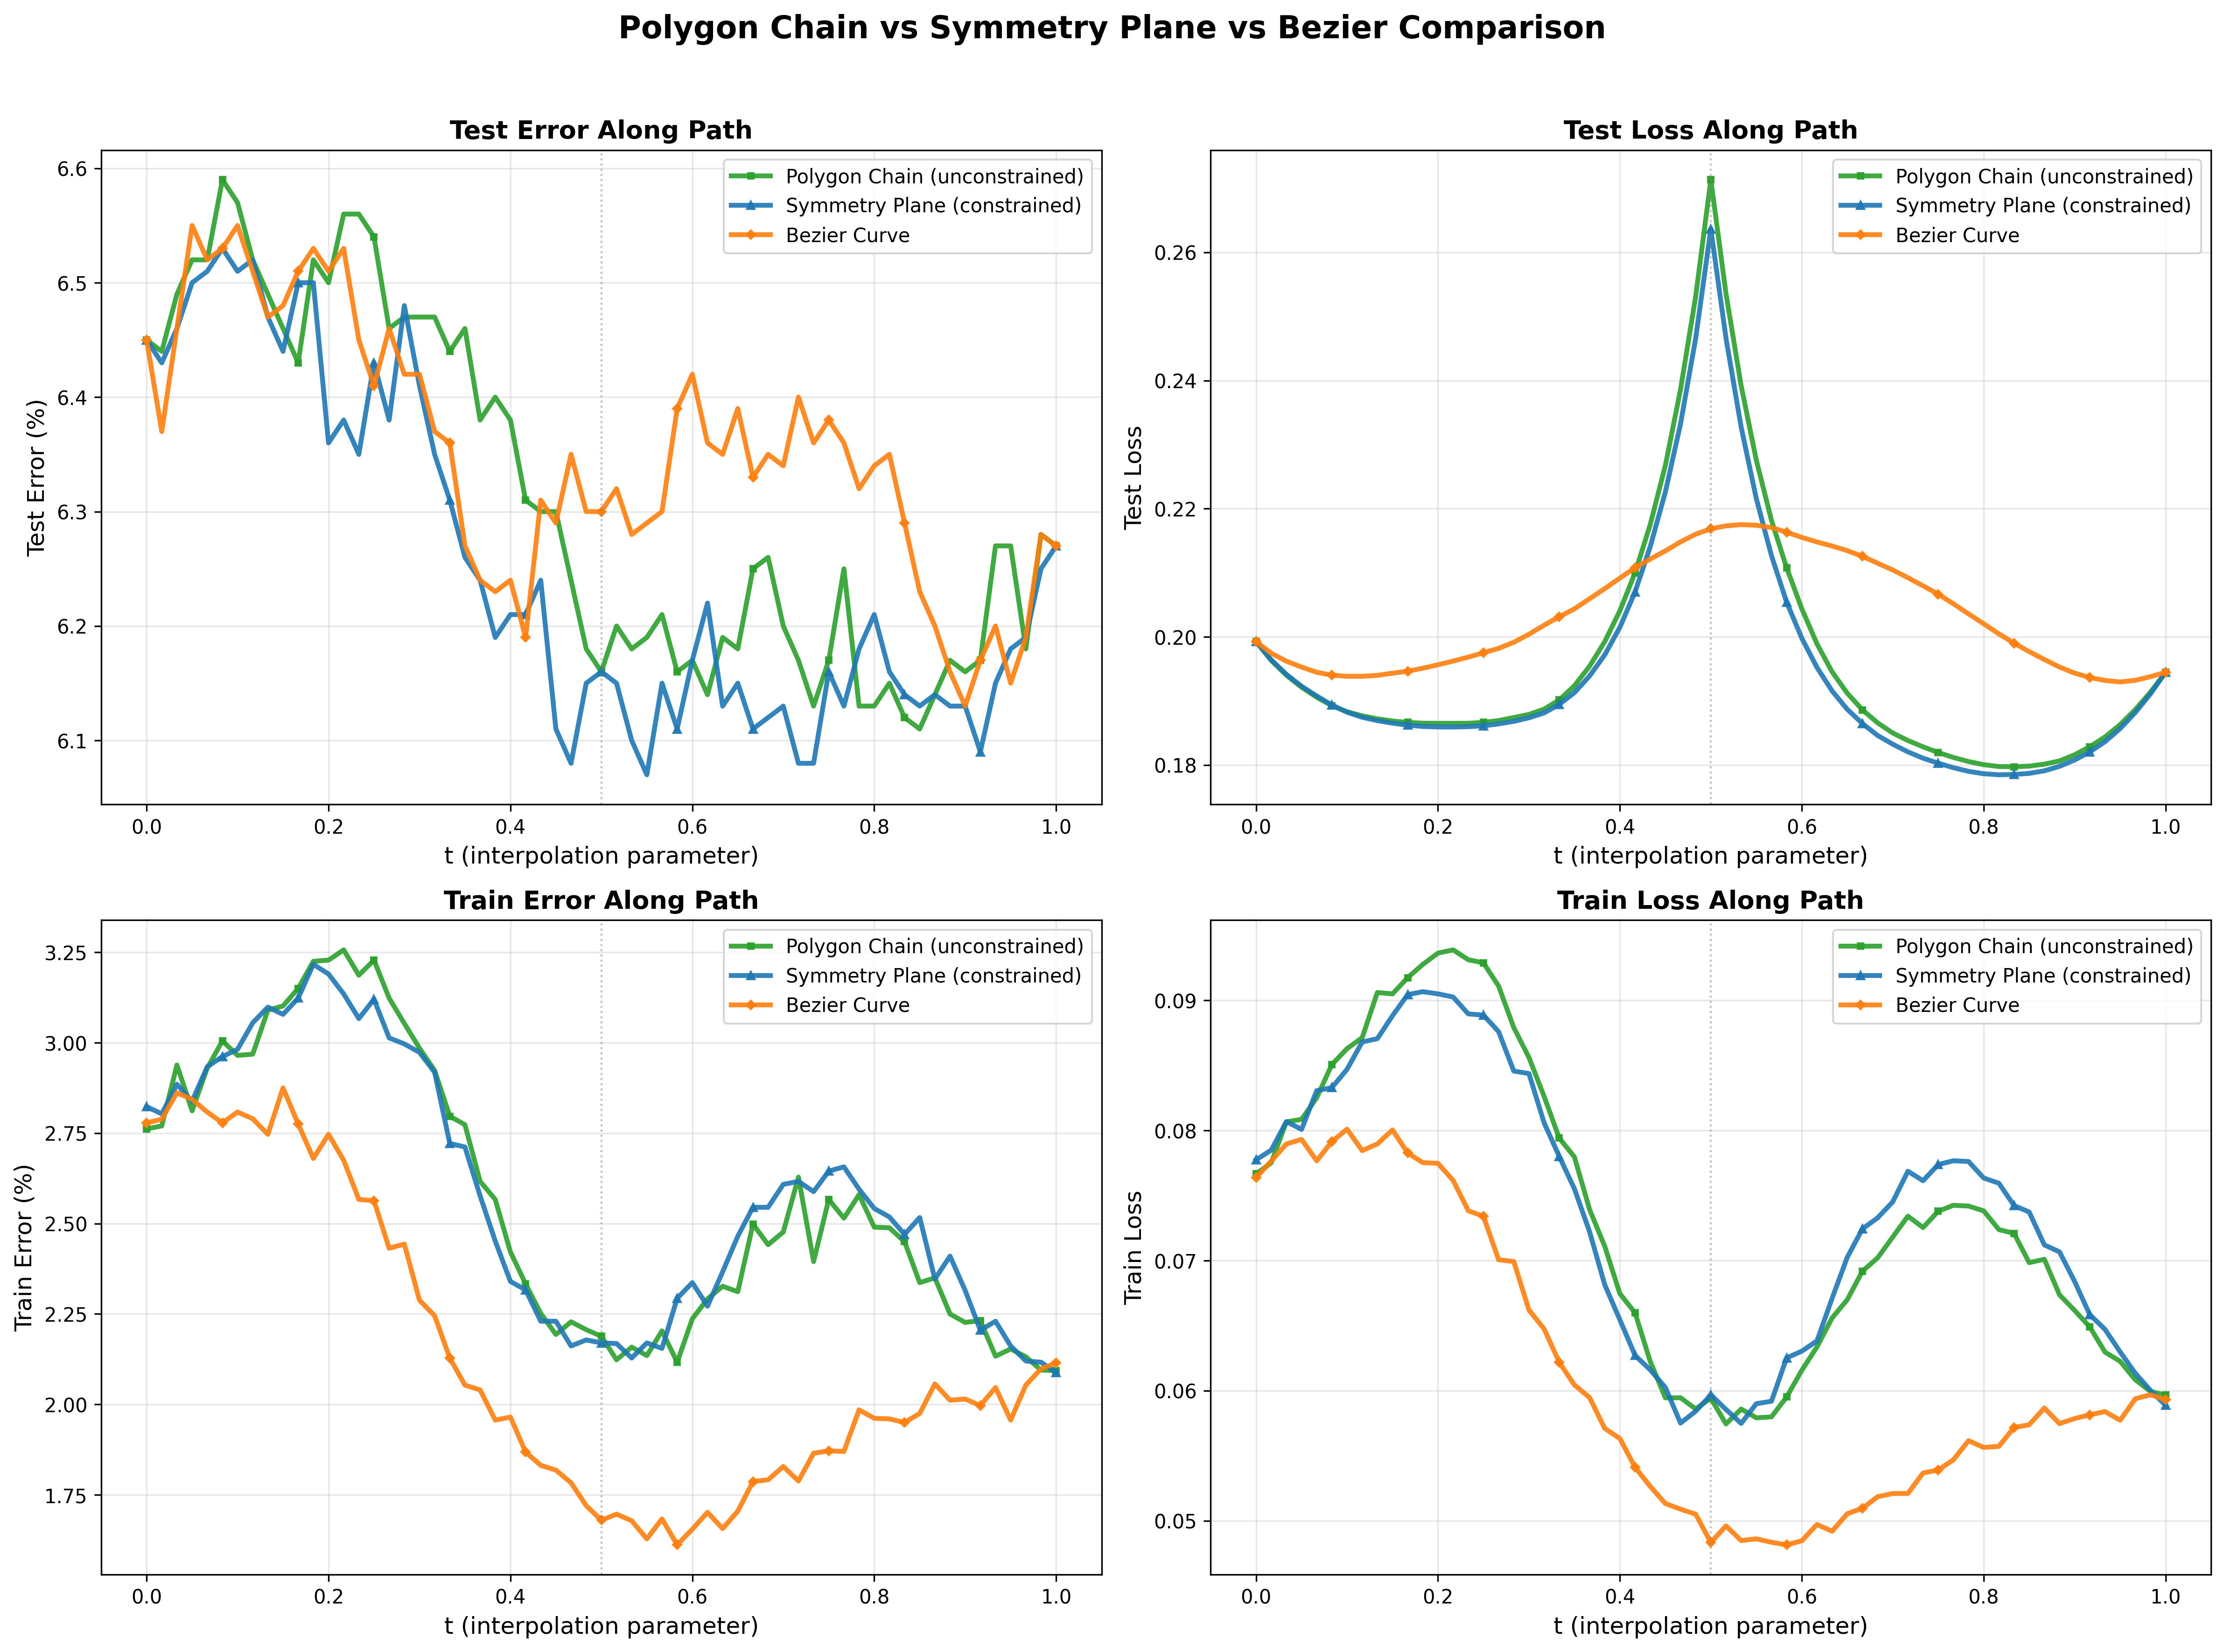
\includegraphics[width=0.95\linewidth]{../draft_3/example_2.png}
    \caption{Loss curves with and without train-time augmentations during evaluation.}
    \label{fig:augmentation_effects}
\end{figure}

The train--test loss gap along the paths is genuine and reflects overfitting in both VGG16/CIFAR-10 and ConvFC/Fashion-MNIST. Train loss curves appear nearly flat when plotted on the same scale as test loss, while test loss varies more strongly along the path. In particular, the midpoint ($t \approx 0.5$) can achieve lower training loss than either endpoint while exhibiting worse test loss, indicating improved fit to training data at the expense of generalization.

\section{Scheduled Experiments}

The following experiments are planned for the remaining thesis period:

\begin{enumerate}
    \item \textbf{Permutation alignment algorithms:} Design, implement, and evaluate neuron alignment methods by:
    \begin{enumerate}
        \item sequentially finding optimal permutations between closely sampled modes along a low-loss path between modes, in order to test whether aligned modes exhibit linear mode connectivity, and comparing against existing alignment methods;
        \item learning, for each layer, a transformation matrix $X$ such that $XW$ maps one mode to another, and then decomposing this transformation into two valid permutation matrices $P_1 W P_2$.
    \end{enumerate}

    \item \textbf{Stronger hyperplane constraints:} Evaluate constraints that remove more than one dimension (e.g., restricting the path to a $k$-dimensional subspace) to identify the dimensionality at which connectivity degrades.


    \item \textbf{Evaluation of existing permutation-finding methods:} Train a mode, transform it so that it represents a different function while remaining in the same linear mode connectivity (LMC) basin, apply a random permutation (ensuring that an optimal permutation exists), and test whether existing permutation alignment methods can successfully recover the correct alignment.

    \item \textbf{Controlled functional-difference benchmark (overlapping Gaussians / noisy XOR):} Create a 2D dataset with intrinsic ambiguity, train many models to similar loss, verify that pairs implement different functions by finding disagreement points, and then test whether alignment methods can recover low-barrier linear connectivity between these genuinely different solutions.
\end{enumerate}


\section{Timeline}
\begin{table}[H]
\centering
\begin{tabular}{l l l}
\toprule
\textbf{Weeks} & \textbf{Activity} & \textbf{Status} \\
\midrule
1--2 & Codebase setup, endpoint training, B\'{e}zier curve experiments & Completed \\
3--4 & Neuron permutation experiments, symmetry plane development & Completed \\
5--8 & Arbitrary hyperplane constraints, initialization experiments & Completed \\
8--10 & ConvFC/Fashion-MNIST validation, evaluation methodology fixes & Completed \\
10 & \textbf{First Stage Evaluation} & \textbf{Current} \\
\midrule
11--13 & Evaluation of existing permutation-finding methods & Planned \\
14--17 & Permutation alignment algorithms, re-evaluation with fixed methodology & Planned \\
18--20 & Stronger hyperplane constraints, scaling experiments & Planned \\
21--30 & Thesis writing & Planned \\
\bottomrule
\end{tabular}
\end{table}


\section{Related Work (Selected)}

\begin{itemize}
    \item \textbf{Draxler et al.\ (2018):} Nudged Elastic Band (NEB) finds low-loss curved paths between minima; does not imply linear connectivity.
    \item \textbf{Garipov et al.\ (2018):} Trainable B\'{e}zier curves connect minima and enable fast geometric ensembling.
    \item \textbf{Frankle et al.\ (2020):} Defined LMC and showed shared-initialization models become linearly connected after short shared training.
    \item \textbf{Entezari et al.\ (2021):} Statistical evidence for LMC modulo permutation; the required permutations are not directly found.
    \item \textbf{Ainsworth et al.\ (2023):} Git Re-Basin alignment methods; strong on wide models, weaker on VGG-style architectures.
    \item \textbf{Jordan et al.\ (2023):} REPAIR shows variance collapse during interpolation and rescales activations to reduce barriers. For interpolated activations $z_t = (1-t)z_A + t z_B$,
    \[
    \mathrm{Var}(z_{0.5}) = \tfrac{1}{4}\mathrm{Var}(z_A) + \tfrac{1}{4}\mathrm{Var}(z_B) + \tfrac{1}{2}\mathrm{Cov}(z_A, z_B),
    \]
    which halves variance when $z_A$ and $z_B$ are uncorrelated.
    \item \textbf{Crisostomi et al.\ (2024):} C$^2$M$^3$ enforces cycle-consistent permutations for multi-model merging.
    \item \textbf{Zhan et al.\ (2025) and Zhao et al.\ (2025):} Theoretical analyses linking width and symmetry (permutation/rescaling) to barrier behavior.
\end{itemize}

\section{References}

\begin{itemize}
    \item Garipov et al.\ (2018): Loss Surfaces, Mode Connectivity, and Fast Ensembling of DNNs.
    \item Draxler et al.\ (2018): Essentially No Barriers in Neural Network Energy Landscape.
    \item Freeman \& Bruna (2017): Topology and Geometry of Half-Rectified Network Optimization.
    \item Entezari et al.\ (2021): The Role of Permutation Invariance in Linear Mode Connectivity of Neural Networks.
    \item Frankle et al.\ (2020): Linear Mode Connectivity and the Lottery Ticket Hypothesis.
    \item Ainsworth et al.\ (2023): Git Re-Basin: Merging Models Modulo Permutation Symmetries.
    \item Jordan et al.\ (2023): REPAIR: REnormalizing Permuted Activations for Interpolation Repair.
    \item Zhan et al.\ (2025): Analyzing the Role of Permutation Invariance in Linear Mode Connectivity.
    \item Zhao et al.\ (2025): Understanding Mode Connectivity via Parameter Space Symmetry.
    \item Crisostomi et al.\ (2024): Cycle-Consistent Multi-Model Merging (C$^2$M$^3$).
\end{itemize}

\end{document}
